\appendix

\chapter{Fichas técnicas y búsqueda en bases de datos}\label{apendice:fichas-y-busquedas}

\section{Ficha técnica del recurso tecnológico}
\begin{figure}[H]
    \centering
    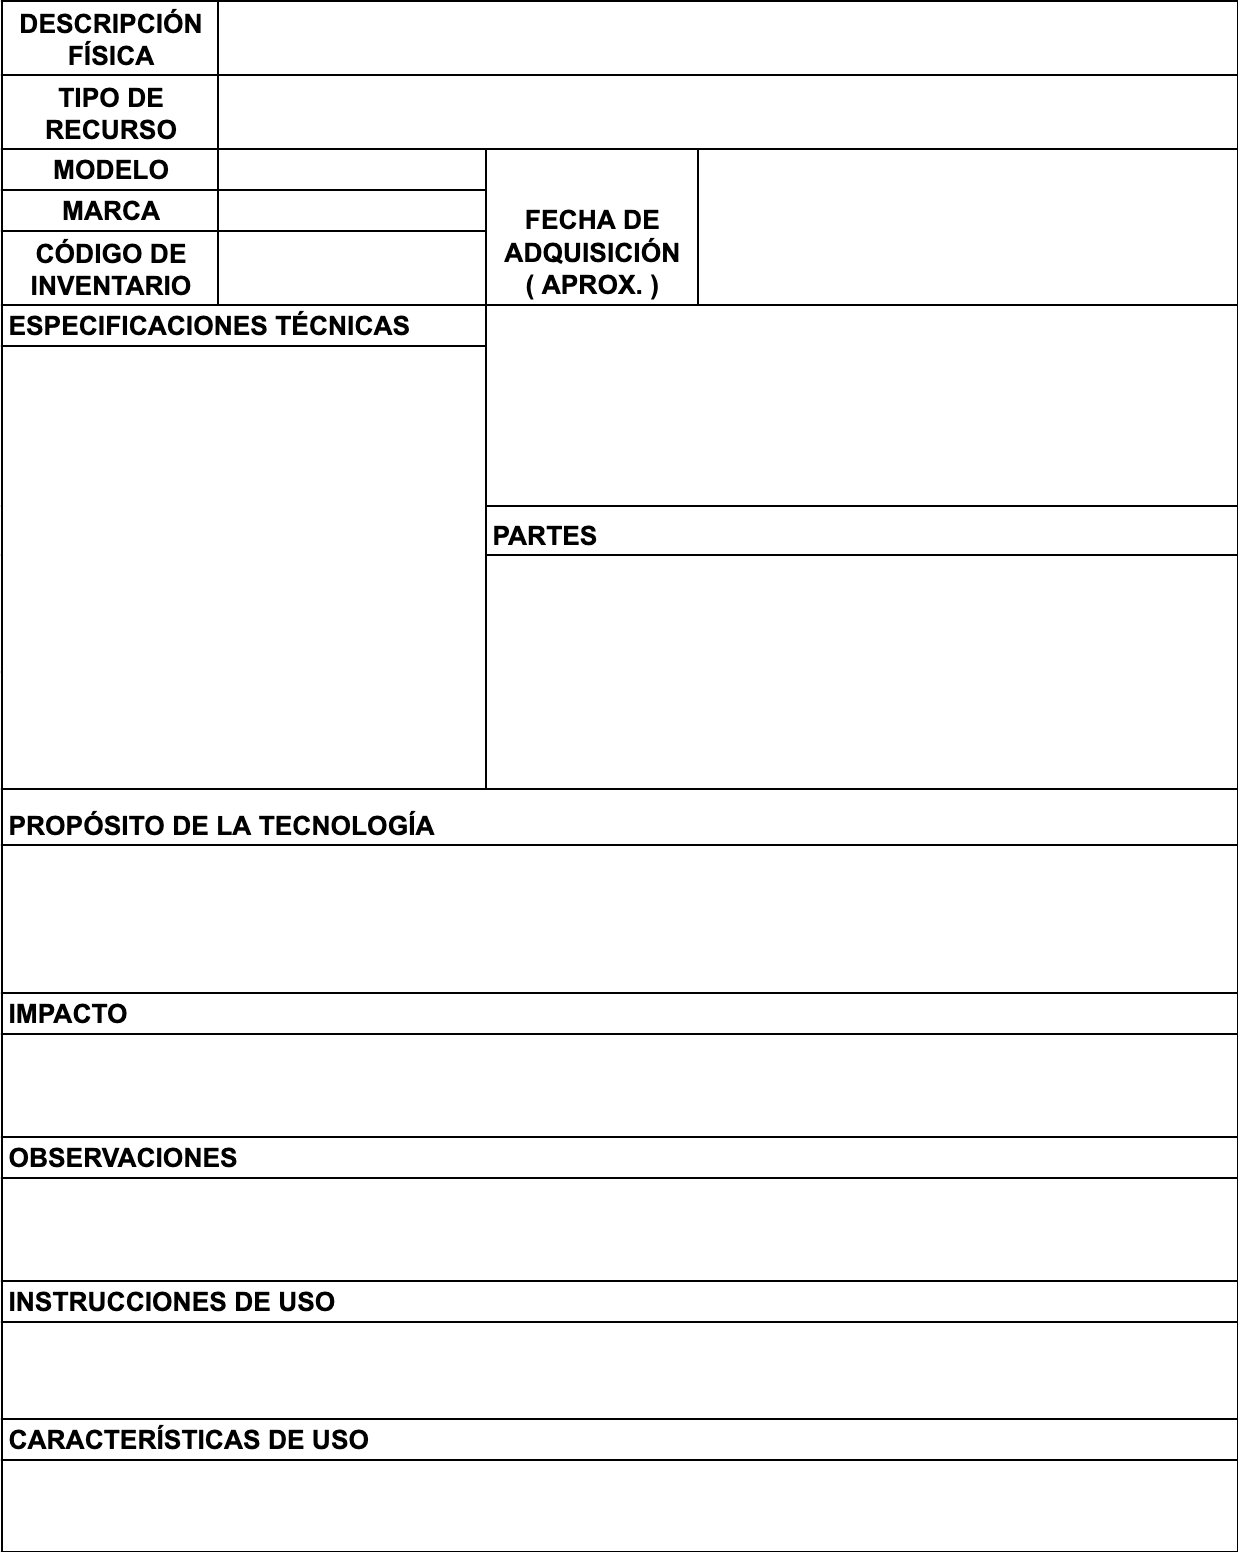
\includegraphics[width=\textwidth,height=0.85\textheight,keepaspectratio]{apendices/caracterizacionInfraestructura.png}
    \caption{Ficha técnica del recurso tecnológico}\label{fig:tabla-ficha-tecnica}
\end{figure}
\FloatBarrier\section*{Ficha técnica de servicios}

\begin{figure}[H]
    \centering
    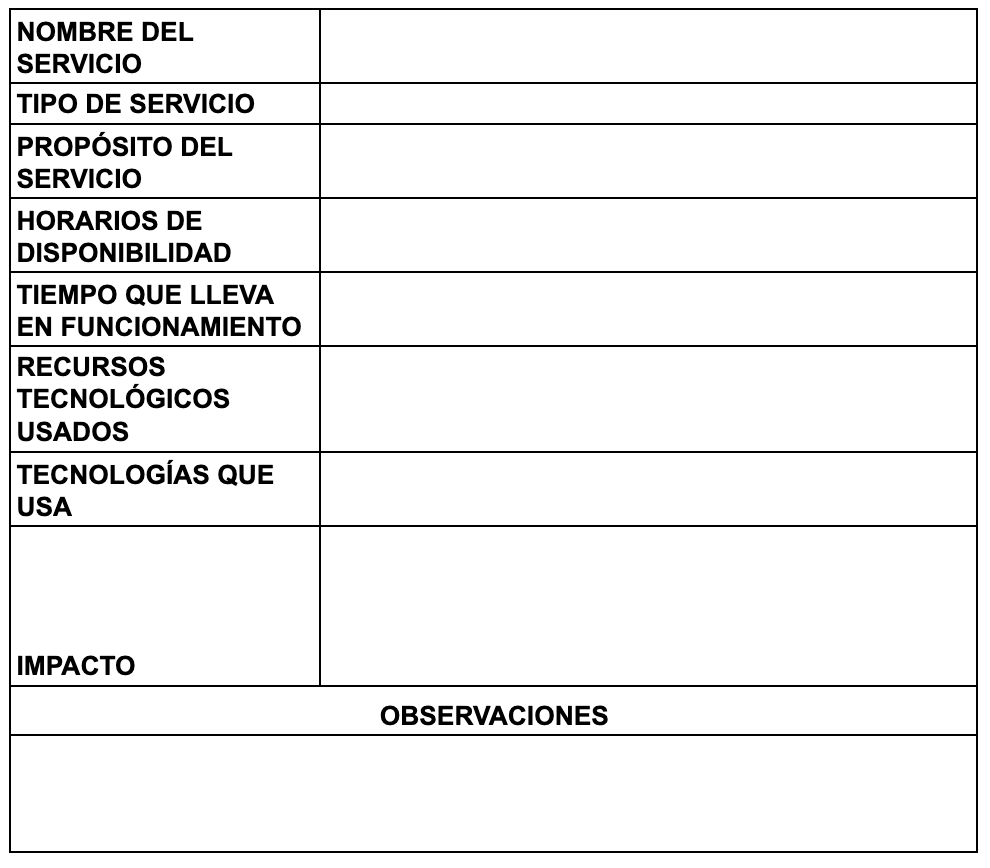
\includegraphics[width=\textwidth,height=0.85\textheight,keepaspectratio]{apendices/caracterizacionServicios.png}
    \caption{Ficha técnica de servicios}\label{fig:tabla-ficha-servicios}
\end{figure}
\FloatBarrier\clearpage

\chapter{Búsquedas en bases de datos}

\section{Cadenas de búsqueda}\label{sec:cadenas-busqueda}


\begin{tcolorbox}[
  colback=gray!5, 
  colframe=black!60, 
  title=Cadena de búsqueda en ACM para educación, 
  fonttitle=\bfseries, 
  sharp corners=south
]
\scriptsize % o \footnotesize, \tiny según lo pequeño que lo quieras
\begin{verbatim}
(Title:("Container-based virtualization" OR "Application virtualization" OR "Docker" OR 
"Lightweight Virtualization") AND Title:("Education" OR "Education System" 
OR "Education Development" OR "Higher Education") ) 

OR

(Abstract:("Container-based virtualization" OR "Application virtualization" OR "Docker"
 OR "Lightweight Virtualization") AND Abstract:("Education" OR "Education System" 
 OR "Education Development" OR "Higher Education") )

OR

(Keyword:("Container-based virtualization" OR "Application virtualization" OR "Docker" OR 
"Lightweight Virtualization")
AND Keyword:("Education" OR "Education System" OR "Education Development" 
OR "Higher Education"))
\end{verbatim}
\end{tcolorbox}

\begin{tcolorbox}[
  colback=gray!5, 
  colframe=black!60, 
  title=Cadena de búsqueda en ACM para investigación, 
  fonttitle=\bfseries, 
  sharp corners=south
]
\scriptsize % puedes usar \tiny para hacerlo aún más pequeño
\begin{verbatim}
(Title:("Container-based virtualization" OR "Application virtualization" OR "Docker" OR 
"Lightweight Virtualization") AND Title:("Research" OR "Research Group" OR 
"Research Proposal"))

OR

(Abstract:("Container-based virtualization" OR "Application virtualization" OR "Docker" OR 
"Lightweight Virtualization") AND Abstract:("Research" OR "Research Group" OR 
"Research Proposal"))

OR

(Keyword:("Container-based virtualization" OR "Application virtualization" OR "Docker" OR 
"Lightweight Virtualization") AND Keyword:("Research" OR "Research Group" OR 
"Research Proposal"))
\end{verbatim}
\end{tcolorbox}

\begin{tcolorbox}[
  colback=gray!5, 
  colframe=black!60, 
  title=Cadena de búsqueda en ACM para extensión, 
  fonttitle=\bfseries, 
  sharp corners=south
]
\scriptsize % puedes usar \tiny para hacerlo aún más pequeño
\begin{verbatim}
(Title:("Container-based virtualization" OR "Application virtualization" OR "Docker" OR 
"Lightweight Virtualization") AND Title:("Industry" OR “IT Services” OR 
“Technology Infrastructure” OR “Cloud Computing”) ) 

OR

(Abstract:("Container-based virtualization" OR "Application virtualization" OR "Docker" 
OR "Lightweight Virtualization") AND Abstract:("Industry" OR “IT Services” OR 
“Technology Infrastructure” OR “Cloud Computing”) )

OR

(Keyword:("Container-based virtualization" OR "Application virtualization" OR "Docker" 
OR "Lightweight Virtualization")
AND Keyword:("Industry" OR “IT Services” OR “Technology Infrastructure” 
OR “Cloud Computing”))

\end{verbatim}
\end{tcolorbox}

\begin{tcolorbox}[
  colback=gray!5, 
  colframe=black!60, 
  title=Cadena de búsqueda en IEE para educación, 
  fonttitle=\bfseries, 
  sharp corners=south
]
\scriptsize % puedes usar \tiny para hacerlo aún más pequeño
\begin{verbatim}
(("Abstract":"Container-based virtualization" OR "Abstract":"Application virtualization" 
OR "Abstract":"Docker" OR "Abstract":"Lightweight Virtualization") AND ("Abstract":"Education" 
OR "Abstract":"Education System" OR "Abstract":"Education Development”  OR 
"Abstract":"Higher Education”)) 

OR (("Publication Title":"Container-based virtualization" OR "Publication 
Title":"Application virtualization" 
OR "Publication Title":"Docker" OR "Publication Title":"Lightweight Virtualization") 
AND ("Publication Title":"Education" 
OR "Publication Title":"Education System" OR "Publication Title":"Education Development”  
OR "Publication Title":"Higher Education” ))

OR (("Author Keywords":"Container-based virtualization" OR 
"Author Keywords":"Application virtualization" OR 
"Author Keywords":"Docker" OR "Author Keywords":"Lightweight Virtualization") AND 
("Author Keywords":"Education" 
OR "Author Keywords":"Education System" OR "Author Keywords":"Education Development”  
OR "Author Keywords":"Higher Education”))
\end{verbatim}
\end{tcolorbox}


\begin{tcolorbox}[
  colback=gray!5, 
  colframe=black!60, 
  title=Cadena de búsqueda en IEE para investigación, 
  fonttitle=\bfseries, 
  sharp corners=south
]
\scriptsize % puedes usar \tiny para hacerlo aún más pequeño
\begin{verbatim}
(("Abstract":"Container-based virtualization" OR "Abstract":"Application virtualization" 
OR "Abstract":"Docker" OR "Abstract":"Lightweight Virtualization") AND 
("Abstract":"Research Group" OR "Abstract":"Research Proposal")) 

OR (("Publication Title":"Container-based virtualization" OR 
"Publication Title":"Application virtualization" OR "Publication Title":"Docker" OR 
"Publication Title":"Lightweight Virtualization") AND 
("Publication Title":"Research Group" OR "Publication Title":"Research Proposal" ))

OR (("Author Keywords":"Container-based virtualization" OR 
"Author Keywords":"Application virtualization" OR "Author Keywords":"Docker" OR 
"Author Keywords":"Lightweight Virtualization") AND 
("Author Keywords":"Research Group" OR "Author Keywords":"Research Proposal"))
\end{verbatim}
\end{tcolorbox}

\begin{tcolorbox}[
  colback=gray!5, 
  colframe=black!60, 
  title=Cadena de búsqueda en IEE para extensión, 
  fonttitle=\bfseries, 
  sharp corners=south
]
\scriptsize % puedes usar \tiny para hacerlo aún más pequeño
\begin{verbatim}
(("Abstract":"Container-based virtualization" OR "Abstract":"Application virtualization" 
OR "Abstract":"Docker" OR "Abstract":"Lightweight Virtualization") AND 
("Abstract":"Industry" OR "Abstract":"IT Services" OR 
"Abstract":"Technology Infrastructure" OR "Abstract":"Cloud Computing")) 

OR (("Publication Title":"Container-based virtualization" OR 
"Publication Title":"Application virtualization" 
OR "Publication Title":"Docker" OR "Publication Title":"Lightweight Virtualization") AND 
("Publication Title":"Industry" OR "Publication Title":"IT Services" OR 
"Publication Title":"Technology Infrastructure" OR "Publication Title":"Cloud Computing"))

OR (("Author Keywords":"Container-based virtualization" OR 
"Author Keywords":"Application virtualization" OR "Author Keywords":"Docker" OR 
"Author Keywords":"Lightweight Virtualization") AND ("Author Keywords":"Industry" OR 
"Author Keywords":"IT Services" OR "Author Keywords":"Technology Infrastructure" OR 
"Author Keywords":"Cloud Computing"))
\end{verbatim}
\end{tcolorbox}

\begin{tcolorbox}[
  colback=gray!5, 
  colframe=black!60, 
  title=Cadena de búsqueda en Springer para educación, 
  fonttitle=\bfseries, 
  sharp corners=south
]
\scriptsize % puedes usar \tiny para hacerlo aún más pequeño
\begin{verbatim}
(title:("Container-based virtualization" OR "Application virtualization" OR 
"Docker" OR "Lightweight Virtualization") AND title:("Education" OR 
"Education System" OR "Education Development" OR "Higher Education"))

OR

(abstract:("Container-based virtualization" OR "Application virtualization" OR 
"Docker" OR "Lightweight Virtualization") AND abstract:("Education" OR 
"Education System" OR "Education Development" OR "Higher Education"))

OR 

(keyword:("Container-based virtualization" OR "Application virtualization" OR 
"Docker" OR "Lightweight Virtualization") AND keyword:("Education" OR 
"Education System" OR "Education Development" OR "Higher Education"))

\end{verbatim}
\end{tcolorbox}

\begin{tcolorbox}[
  colback=gray!5, 
  colframe=black!60, 
  title=Cadena de búsqueda en Springer para investigación, 
  fonttitle=\bfseries, 
  sharp corners=south
]
\scriptsize % puedes usar \tiny para hacerlo aún más pequeño
\begin{verbatim}
(title:("Container-based virtualization" OR "Application virtualization" OR 
"Docker" OR "Lightweight Virtualization") AND title:("research" OR 
"Research Group" OR "Research Proposal"))

OR

(abstract:("Container-based virtualization" OR "Application virtualization" 
OR "Docker" OR "Lightweight Virtualization") AND abstract:("research" 
OR "Research Group" OR "Research Proposal"))

OR 

(keyword:("Container-based virtualization" OR "Application virtualization"
 OR "Docker" OR "Lightweight Virtualization") AND keyword:("research" OR 
 "Research Group" OR "Research Proposal"))

\end{verbatim}
\end{tcolorbox}

\begin{tcolorbox}[
  colback=gray!5, 
  colframe=black!60, 
  title=Cadena de búsqueda en Springer para extensión, 
  fonttitle=\bfseries, 
  sharp corners=south
]
\scriptsize % puedes usar \tiny para hacerlo aún más pequeño
\begin{verbatim}
(title:("Container-based virtualization" OR "Application virtualization"
 OR "Docker" OR "Lightweight Virtualization") AND title:("Industry" OR 
 “IT Services” OR “Technology Infrastructure” OR “Cloud Computing”))

OR

(abstract:("Container-based virtualization" OR "Application virtualization" 
OR "Docker" OR "Lightweight Virtualization") AND abstract:("Industry" OR 
“IT Services” OR “Technology Infrastructure” OR “Cloud Computing”))

OR 

(keyword:("Container-based virtualization" OR "Application virtualization"
 OR "Docker" OR "Lightweight Virtualization") AND keyword:("Industry" 
 OR “IT Services” OR “Technology Infrastructure” OR “Cloud Computing”))

\end{verbatim}
\end{tcolorbox}

\begin{tcolorbox}[
  colback=gray!5, 
  colframe=black!60, 
  title=Cadena de búsqueda en Science Direct para educación, 
  fonttitle=\bfseries, 
  sharp corners=south
]
\scriptsize % puedes usar \tiny para hacerlo aún más pequeño
\begin{verbatim}
("Container-based virtualization" OR "Application virtualization" 
OR "Docker" OR "Lightweight Virtualization")  AND ("Education" OR 
"Education System" OR "Education Development" OR "Higher Education")
\end{verbatim}
\end{tcolorbox}


\begin{tcolorbox}[
  colback=gray!5, 
  colframe=black!60, 
  title=Cadena de búsqueda en Science Direct para investigación, 
  fonttitle=\bfseries, 
  sharp corners=south
]
\scriptsize % puedes usar \tiny para hacerlo aún más pequeño
\begin{verbatim}
("Container-based virtualization" OR "Application virtualization" OR 
"Docker" OR "Lightweight Virtualization")  AND ("Research" OR 
"Research Group" OR "Research Proposal")
\end{verbatim}
\end{tcolorbox}

\begin{tcolorbox}[
  colback=gray!5, 
  colframe=black!60, 
  title=Cadena de búsqueda en Science Direct para extensión, 
  fonttitle=\bfseries, 
  sharp corners=south
]
\scriptsize % puedes usar \tiny para hacerlo aún más pequeño
\begin{verbatim}
("Container-based virtualization" OR "Application virtualization" OR "Docker" OR 
"Lightweight Virtualization")  AND 
(“Industry” OR "IT Services" OR "Technology Infrastructure" OR "Cloud Computing")
\end{verbatim}
\end{tcolorbox}

\begin{tcolorbox}[
  colback=gray!5, 
  colframe=black!60, 
  title=Cadena de búsqueda en Taylor \& Francis para educación, 
  fonttitle=\bfseries, 
  sharp corners=south
]
\scriptsize % puedes usar \tiny para hacerlo aún más pequeño
\begin{verbatim}
("Application virtualization" OR "Docker" OR "Lightweight Virtualization" OR "Docker Container")   
AND   
("Education System" OR "Education Sector" OR "Education Development" OR "Higher Education")
\end{verbatim}
\end{tcolorbox}

\begin{tcolorbox}[
  colback=gray!5, 
  colframe=black!60, 
  title=Cadena de búsqueda en Taylor \& Francis para investigación, 
  fonttitle=\bfseries, 
  sharp corners=south
]
\scriptsize % puedes usar \tiny para hacerlo aún más pequeño
\begin{verbatim}
("Application virtualization" OR "Docker" OR "Lightweight Virtualization" OR "Docker Container")
AND   
("Specific Research Areas" OR "Research Group" OR "Research Proposal" OR "Research and Development")
\end{verbatim}
\end{tcolorbox}

\begin{tcolorbox}[
  colback=gray!5, 
  colframe=black!60, 
  title=Cadena de búsqueda en Taylor \& Francis para extensión, 
  fonttitle=\bfseries, 
  sharp corners=south
]
\scriptsize % puedes usar \tiny para hacerlo aún más pequeño
\begin{verbatim}
("Application virtualization" OR "Docker" OR "Lightweight Virtualization" OR "Docker Container")  
AND 
(“Industry” OR "IT Services" OR "Technology Infrastructure" OR "Cloud Computing")
\end{verbatim}
\end{tcolorbox}


\section{Búsqueda de artículos sin criterios de inclusión/exclusión}

\begin{figure}[H]
    \centering
    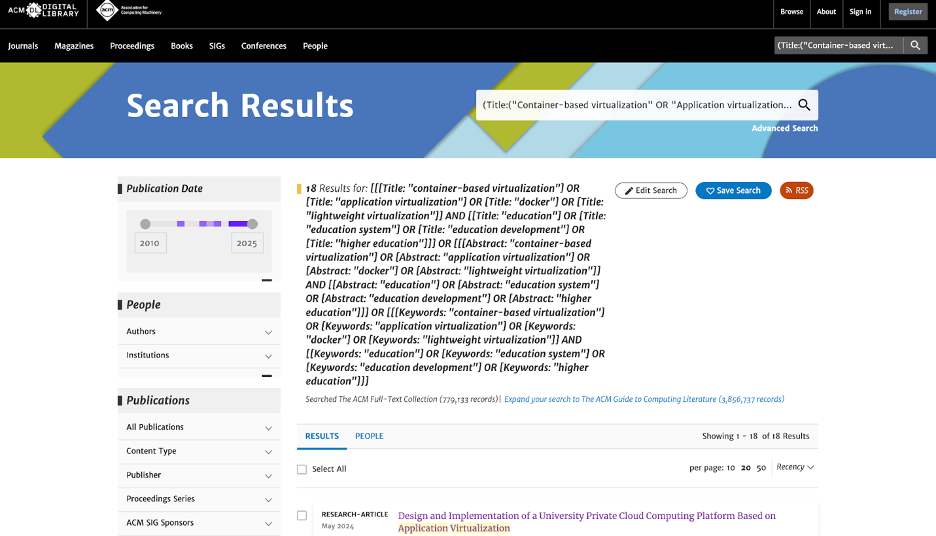
\includegraphics[width=\textwidth,keepaspectratio]{apendices/BD/sin-criterios/ACM-ed.png}
    \caption{Búsqueda de artículos de educación en ACM sin criterios de inclusión/exclusión \\
    Fecha de acceso: 12/03/25 9:13 pm
    }\label{fig:busqueda1}
\end{figure}
\FloatBarrier\begin{figure}[H]
    \centering
    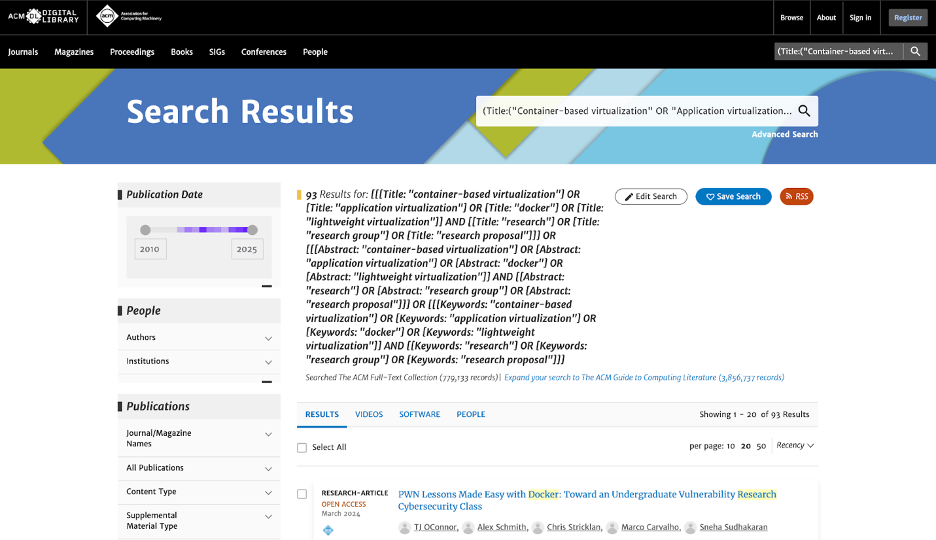
\includegraphics[width=\textwidth,keepaspectratio]{apendices/BD/sin-criterios/ACM-inv.png}
    \caption{Búsqueda de artículos de investigación en ACM sin criterios de inclusión/exclusión \\
    Fecha de acceso: 12/03/25 8:23 pm
    }\label{fig:busqueda2}
\end{figure}
\FloatBarrier\begin{figure}[H]
    \centering
    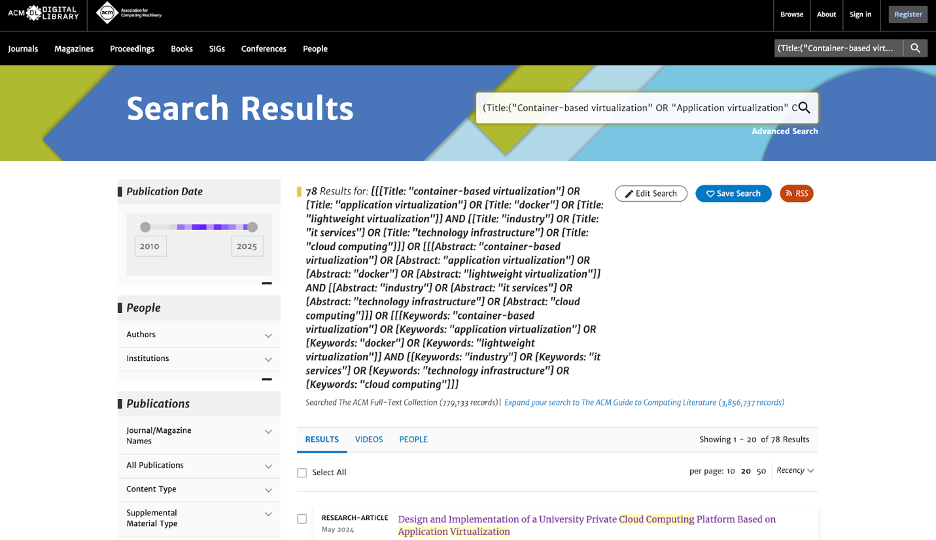
\includegraphics[width=\textwidth,keepaspectratio]{apendices/BD/sin-criterios/ACM-ind.png}
    \caption{Búsqueda de artículos de extensión en ACM sin criterios de inclusión/exclusión \\
    Fecha de acceso: 12/03/25 9:20 pm
    }\label{fig:busqueda3}
\end{figure}
\FloatBarrier\begin{figure}[H]
    \centering
    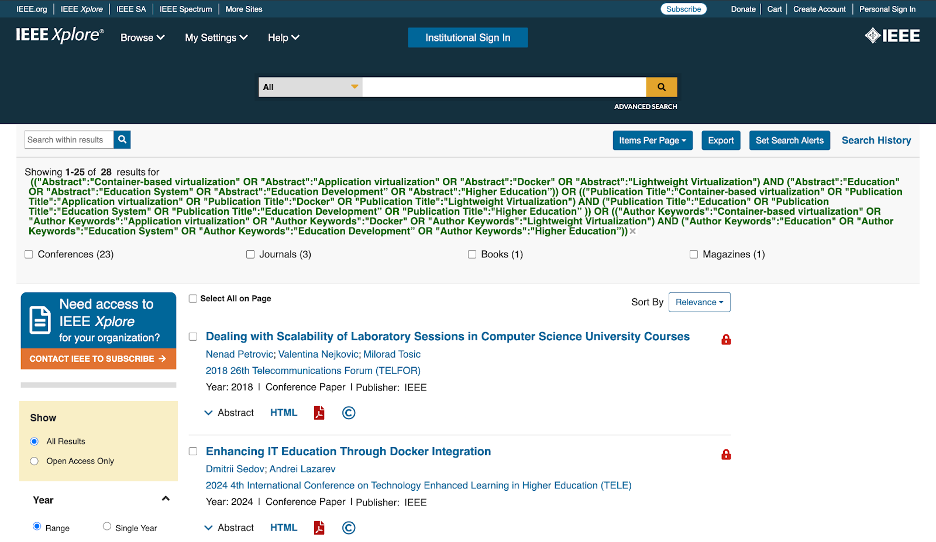
\includegraphics[width=\textwidth,keepaspectratio]{apendices/BD/sin-criterios/IEEE-ed.png}
    \caption{Búsqueda de artículos de educación en IEEE sin criterios de inclusión/exclusión
    Fecha de acceso: 7/03/25 8:50 pm
    }\label{fig:busqueda4}
\end{figure}
\FloatBarrier\begin{figure}[H]
    \centering
    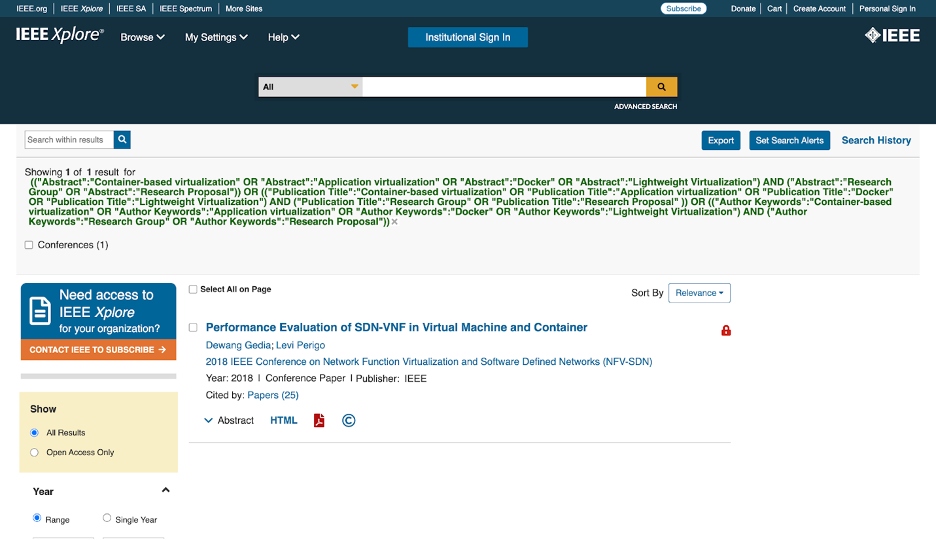
\includegraphics[width=\textwidth,keepaspectratio]{apendices/BD/sin-criterios/IEEE-inv.png}
    \caption{Búsqueda de artículos de investigación en IEEE sin criterios de inclusión/exclusión
    Fecha de acceso: 7/03/25 8:46 pm
    }\label{fig:busqueda5}
\end{figure}
\FloatBarrier\begin{figure}[H]
    \centering
    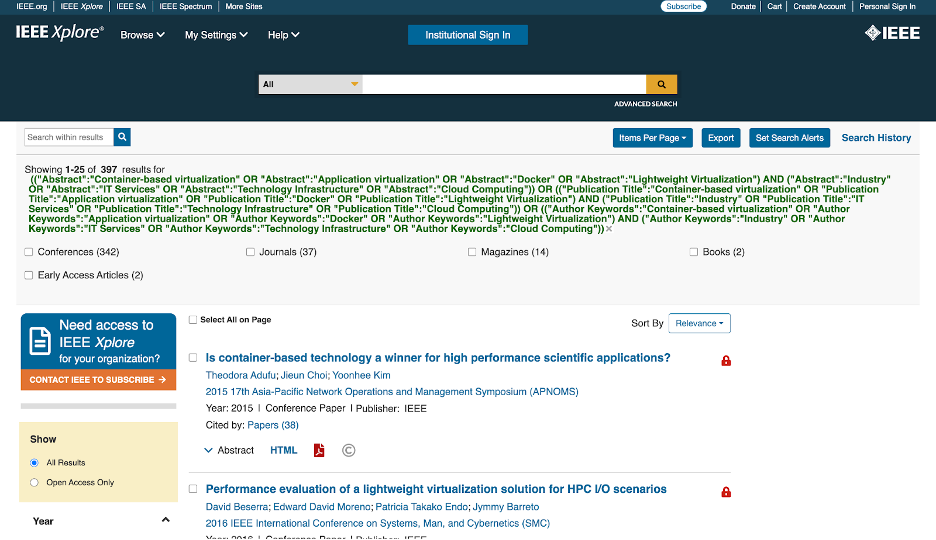
\includegraphics[width=\textwidth,keepaspectratio]{apendices/BD/sin-criterios/IEEE-ind.png}
    \caption{Búsqueda de artículos de extensión en IEEE sin criterios de inclusión/exclusión
    Fecha de acceso: 12/03/25 8:54 pm
    }\label{fig:busqueda6}
\end{figure}
\FloatBarrier\begin{figure}[H]
    \centering
    \includegraphics[width=\textwidth,keepaspectratio]{apendices/BD/sin-criterios/Springer-ed.png}
    \caption{Búsqueda de artículos de educación en Springer sin criterios de inclusión/exclusión
    Fecha de acceso: 12/03/25 9:58 pm
    }\label{fig:busqueda7}
\end{figure}
\FloatBarrier\begin{figure}[H]
    \centering
    \includegraphics[width=\textwidth,keepaspectratio]{apendices/BD/sin-criterios/Springer-inv.png}
    \caption{Búsqueda de artículos de investigación en Springer sin criterios de inclusión/exclusión
    Fecha de acceso: 13/03/25 12:40 pm
    }\label{fig:busqueda8}
\end{figure}
\FloatBarrier\begin{figure}[H]
    \centering
    \includegraphics[width=\textwidth,keepaspectratio]{apendices/BD/sin-criterios/Springer-ind.png}
    \caption{Búsqueda de artículos de extensión en Springer sin criterios de inclusión/exclusión
    Fecha de acceso: 13/03/25 12:48 pm}\label{fig:busqueda9}
\end{figure}
\FloatBarrier\begin{figure}[H]
    \centering
    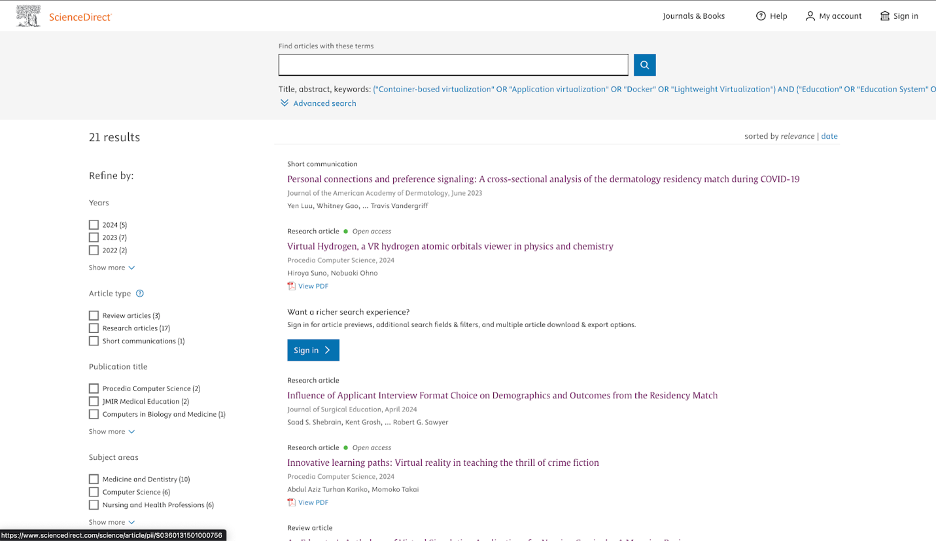
\includegraphics[width=\textwidth,keepaspectratio]{apendices/BD/sin-criterios/SD-ed.png}
    \caption{Búsqueda de artículos de educación en Science Direct sin criterios de inclusión/exclusión
    Fecha de acceso: 13/03/25 1:03 pm}\label{fig:busqueda10}
\end{figure}
\FloatBarrier\begin{figure}[H]
    \centering
    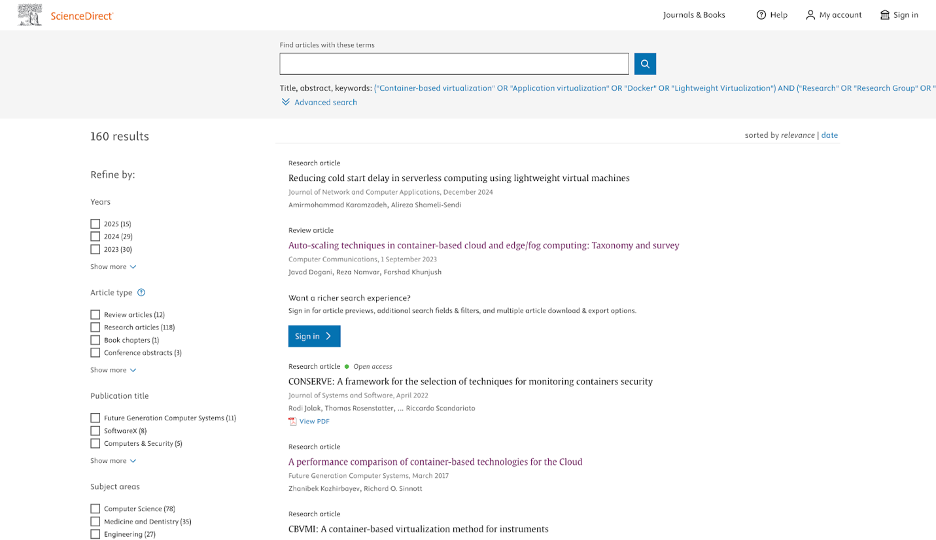
\includegraphics[width=\textwidth,keepaspectratio]{apendices/BD/sin-criterios/SD-inv.png}
    \caption{Búsqueda de artículos de investigación en Science Direct sin criterios de inclusión/exclusión
    Fecha de acceso: 13/03/25 1:43 pm}\label{fig:busqueda11}
\end{figure}
\FloatBarrier\begin{figure}[H]
    \centering
    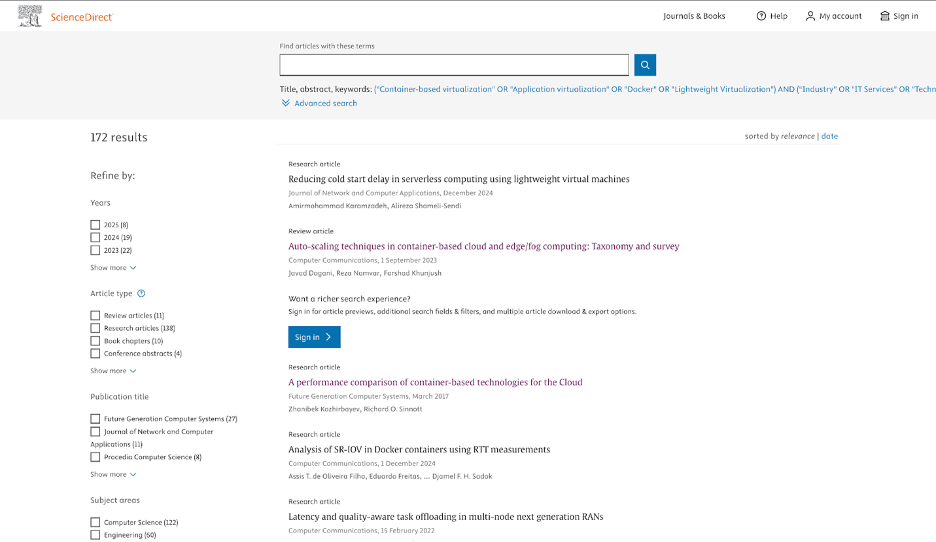
\includegraphics[width=\textwidth,keepaspectratio]{apendices/BD/sin-criterios/SD-ind.png}
    \caption{Búsqueda de artículos de extensión en Science Direct sin criterios de inclusión/exclusión
    Fecha de acceso: 13/03/25 1:48 pm}\label{fig:busqueda12}
\end{figure}
\FloatBarrier\begin{figure}[H]
    \centering
    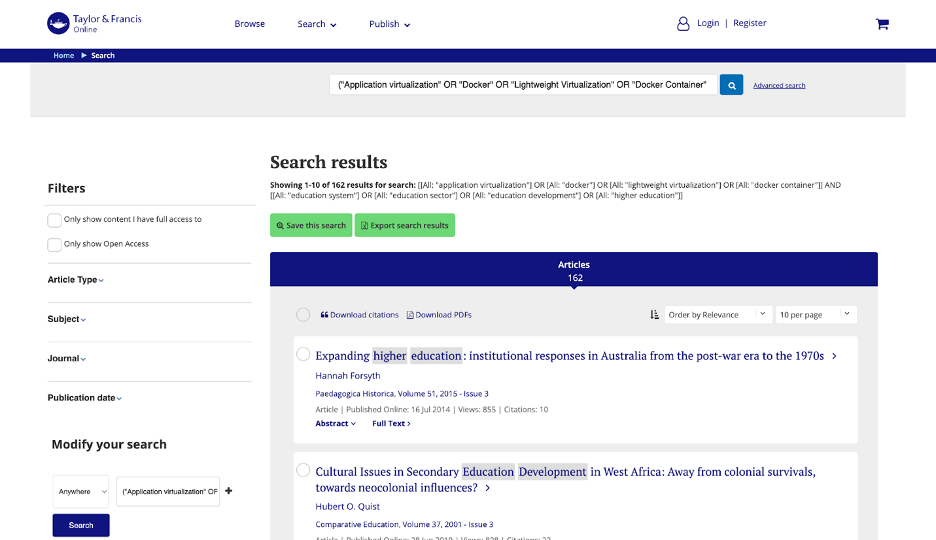
\includegraphics[width=\textwidth,keepaspectratio]{apendices/BD/sin-criterios/TF-ed.png}
    \caption{Búsqueda de artículos de educación en Taylor \& Francis sin criterios de inclusión/exclusión
    Fecha de acceso: 16/03/25 9:21 pm}\label{fig:busqueda13}
\end{figure}
\FloatBarrier\begin{figure}[H]
    \centering
    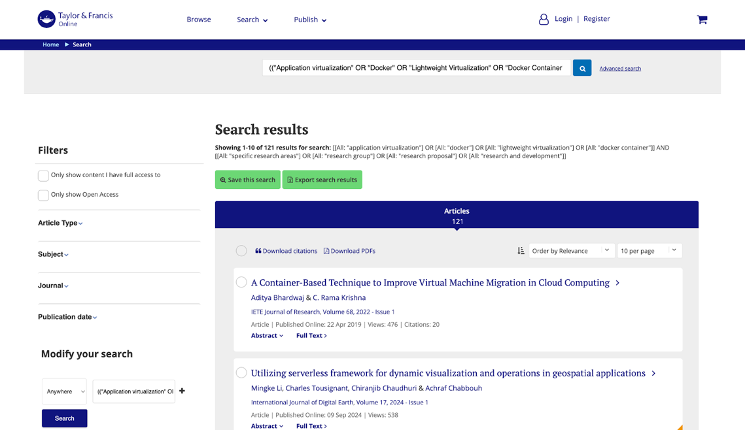
\includegraphics[width=\textwidth,keepaspectratio]{apendices/BD/sin-criterios/TF-inv.png}
    \caption{Búsqueda de artículos de investigación en Taylor \& Francis sin criterios de inclusión/exclusión
    Fecha de acceso: 16/03/25 9:31 pm
    }\label{fig:busqueda14}
\end{figure}
\FloatBarrier\begin{figure}[H]
    \centering
    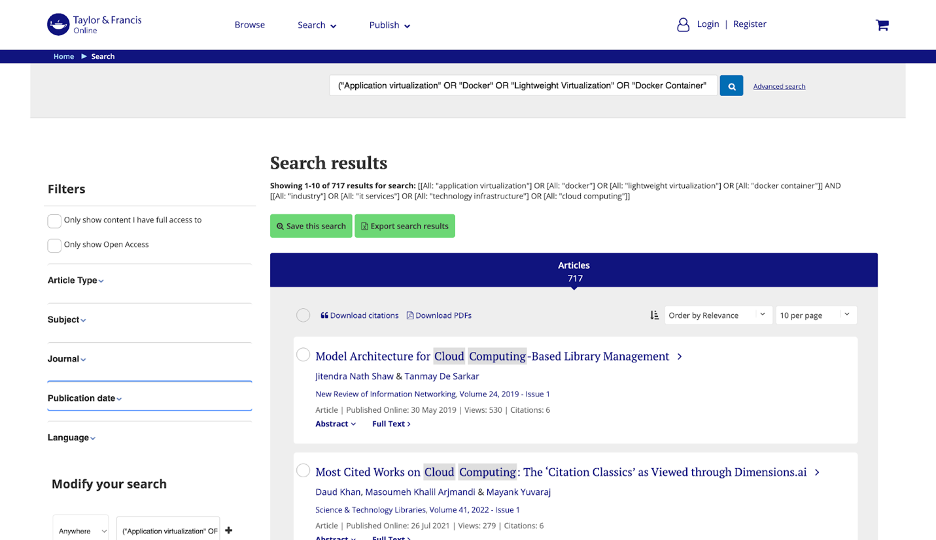
\includegraphics[width=\textwidth,keepaspectratio]{apendices/BD/sin-criterios/TF-ind.png}
    \caption{Búsqueda de artículos de extensión en Taylor \& Francis sin criterios de inclusión/exclusión
    Fecha de acceso: 16/03/25 9:34 pm
    }\label{fig:busqueda15}
\end{figure}
\FloatBarrier\section{Búsqueda de artículos usando criterios de inclusión/exclusión}
\begin{figure}[H]
    \centering
    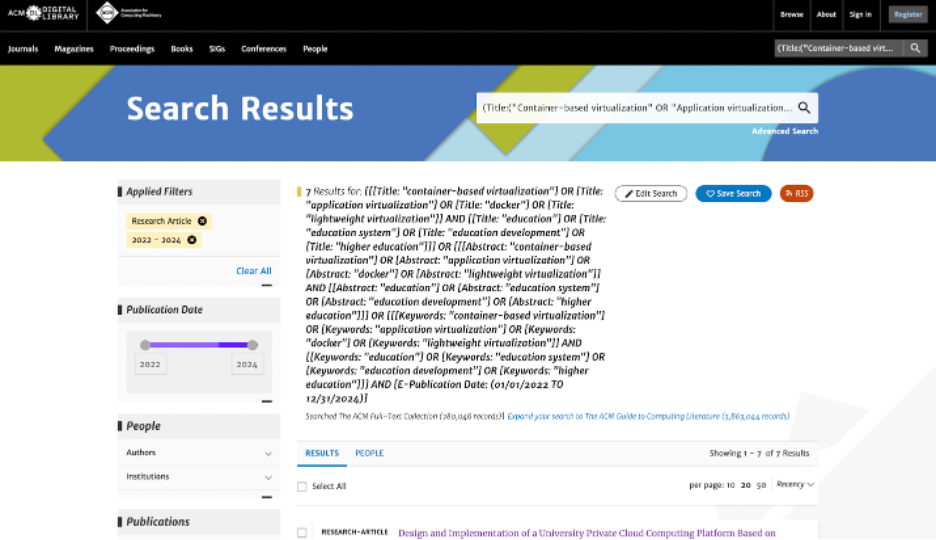
\includegraphics[width=\textwidth,keepaspectratio]{apendices/BD/criterios/ACM-ed.png}
    \caption{Búsqueda de artículos de educación en ACM con criterios de inclusión/exclusión
    Fecha de acceso: 20/03/25 1:15 pm
    }\label{fig:busqueda16}
\end{figure}
\FloatBarrier\begin{figure}[H]
    \centering
    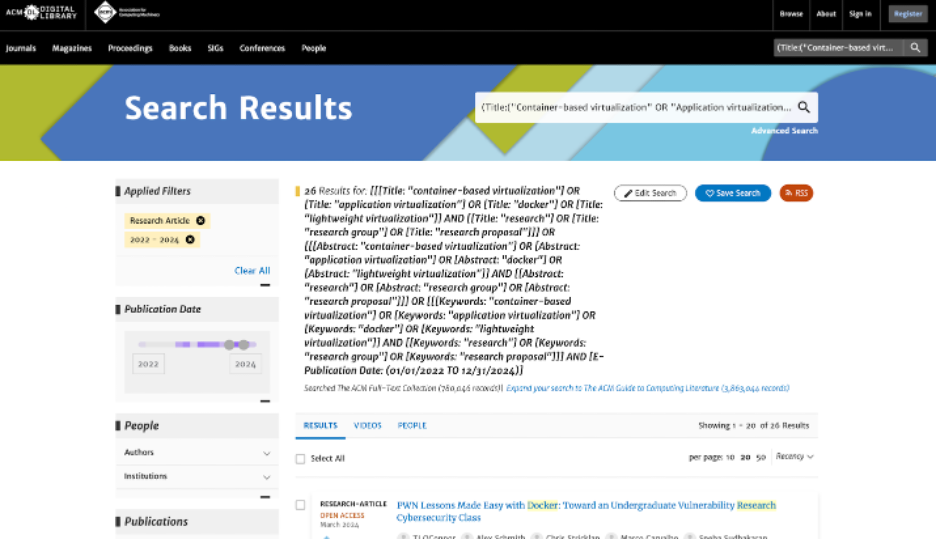
\includegraphics[width=\textwidth,keepaspectratio]{apendices/BD/criterios/ACM-inv.png}
    \caption{Búsqueda de artículos de investigación en ACM con criterios de inclusión/exclusión
    Fecha de acceso: 20/03/25 1:19 pm
    }\label{fig:busqueda17}
\end{figure}
\FloatBarrier\begin{figure}[H]
    \centering
    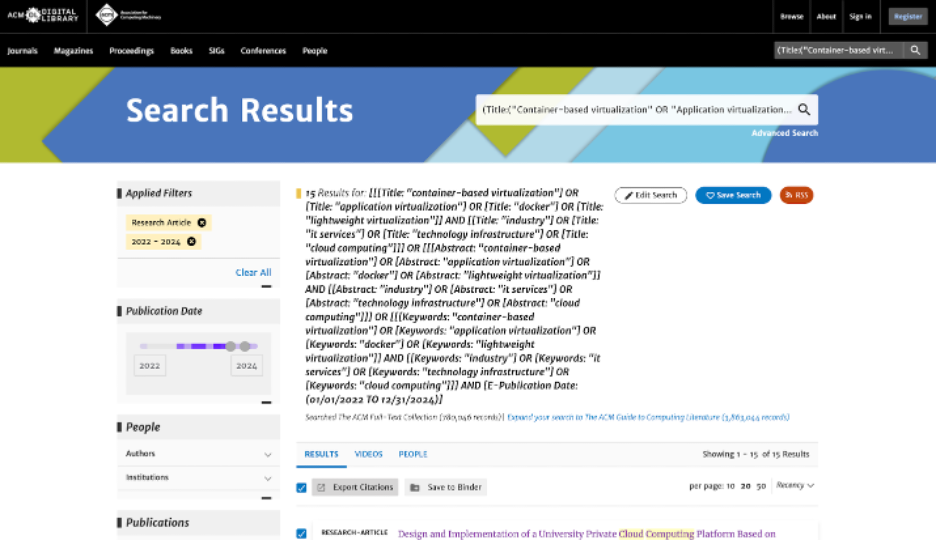
\includegraphics[width=\textwidth,keepaspectratio]{apendices/BD/criterios/ACM-ind.png}
    \caption{Búsqueda de artículos de extensión en ACM con criterios de inclusión/exclusión
    Fecha de acceso: 20/03/25 1:20 pm
    }\label{fig:busqueda18}
\end{figure}
\FloatBarrier\begin{figure}[H]
    \centering
    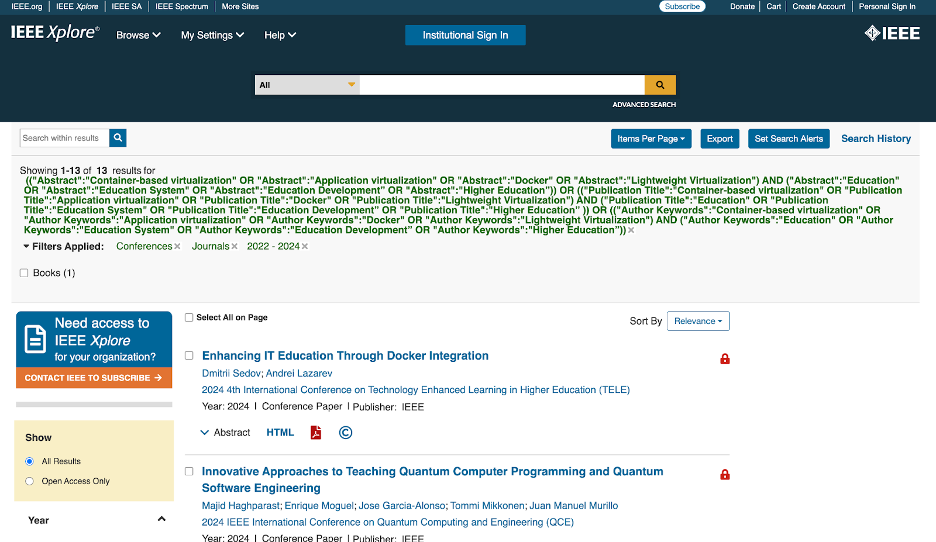
\includegraphics[width=\textwidth,keepaspectratio]{apendices/BD/criterios/IEEE-ed.png}
    \caption{Búsqueda de artículos de educación en IEEE con criterios de inclusión/exclusión
    Fecha de acceso: 20/03/25 1:27 pm
    }\label{fig:busqueda19}
\end{figure}
\FloatBarrier\begin{figure}[H]
    \centering
    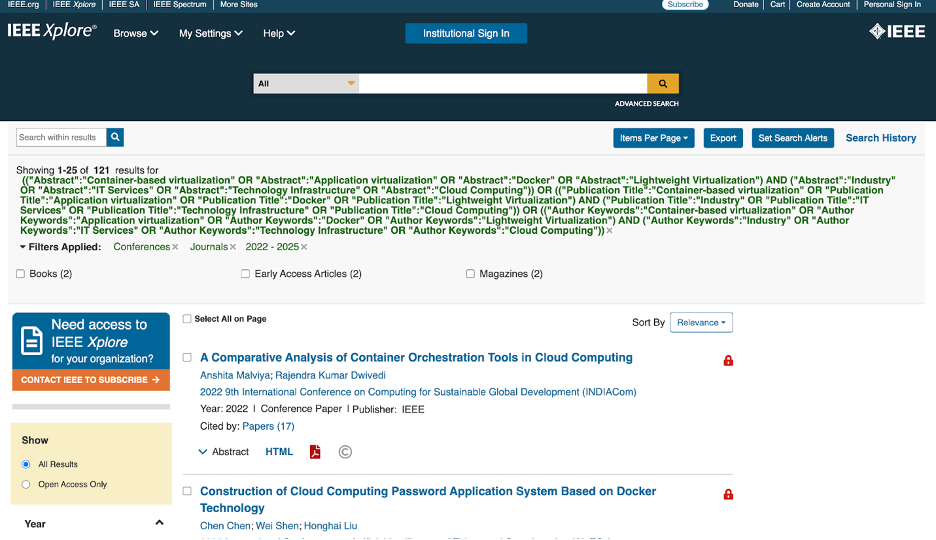
\includegraphics[width=\textwidth,keepaspectratio]{apendices/BD/criterios/IEEE-ind.png}
    \caption{Búsqueda de artículos de extensión en IEEE con criterios de inclusión/exclusión
    Fecha de acceso: 20/03/25 1:37 pm
    }\label{fig:busqueda21}
\end{figure}
\FloatBarrier\begin{figure}[H]
    \centering
    \includegraphics[width=\textwidth,keepaspectratio]{apendices/BD/criterios/Springer-ed.png}
    \caption{Búsqueda de artículos de educación en Springer con criterios de inclusión/exclusión
    Fecha de acceso: 20/03/25 2:29 pm
    }\label{fig:busqueda22}
\end{figure}
\FloatBarrier\begin{figure}[H]
    \centering
    \includegraphics[width=\textwidth,keepaspectratio]{apendices/BD/criterios/Springer-inv.png}
    \caption{Búsqueda de artículos de investigación en Springer con criterios de inclusión/exclusión
    Fecha de acceso: 16/03/25 11:05 am
    }\label{fig:busqueda23}
\end{figure}
\FloatBarrier\begin{figure}[H]
    \centering
    \includegraphics[width=\textwidth,keepaspectratio]{apendices/BD/criterios/Springer-ind.png}
    \caption{Búsqueda de artículos de extensión en Springer con criterios de inclusión/exclusión
    Fecha de acceso: 16/03/25 11:07 am
    }\label{fig:busqueda24}
\end{figure}
\FloatBarrier\begin{figure}[H]
    \centering
    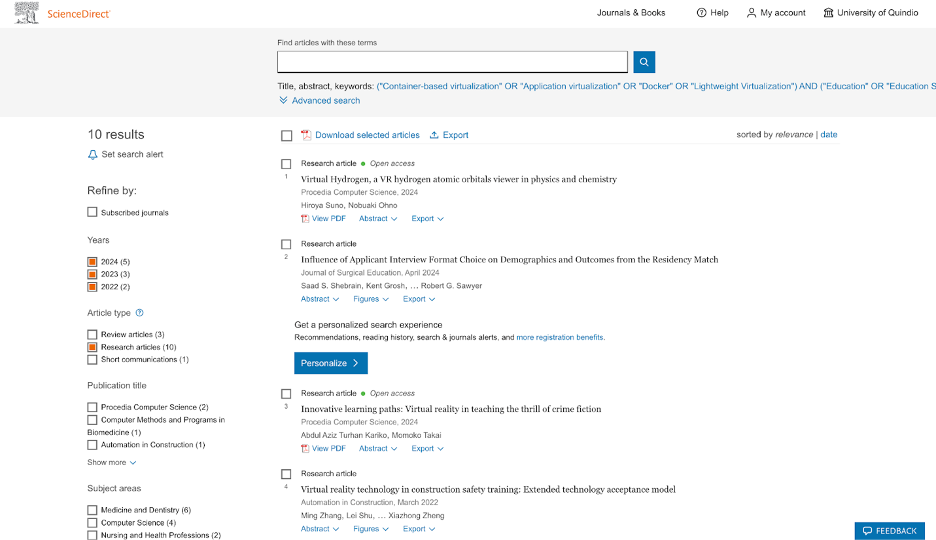
\includegraphics[width=\textwidth,keepaspectratio]{apendices/BD/criterios/SD-ed.png}
    \caption{Búsqueda de artículos de educación en Science Direct con criterios de inclusión/exclusión
    Fecha de acceso: 20/03/25 2:59 am
    }\label{fig:busqueda25}
\end{figure}
\FloatBarrier\begin{figure}[H]
    \centering
    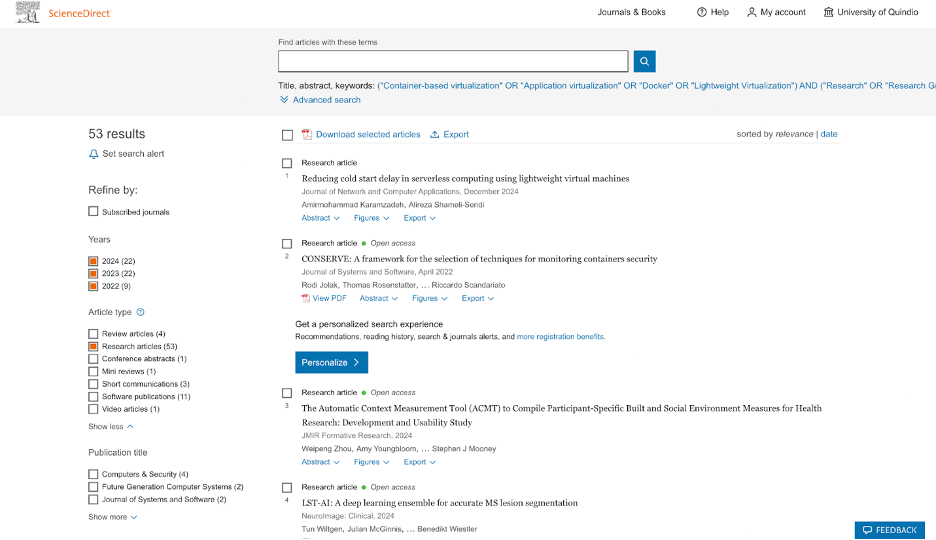
\includegraphics[width=\textwidth,keepaspectratio]{apendices/BD/criterios/SD-inv.png}
    \caption{Búsqueda de artículos de investigación en Science Direct con criterios de inclusión/exclusión
    Fecha de acceso: 20/03/25 3:01 am
    }\label{fig:busqueda26}
\end{figure}
\FloatBarrier\begin{figure}[H]
    \centering
    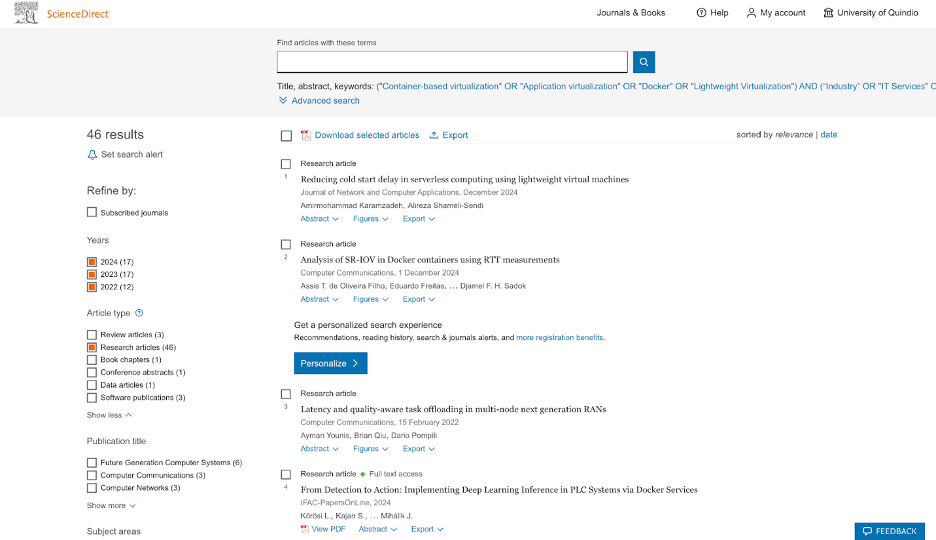
\includegraphics[width=\textwidth,keepaspectratio]{apendices/BD/criterios/SD-ind.png}
    \caption{Búsqueda de artículos de extensión en Science Direct con criterios de inclusión/exclusión
    Fecha de acceso: 20/03/25 3:07 am
    }\label{fig:busqueda27}
\end{figure}
\FloatBarrier\begin{figure}[H]
    \centering
    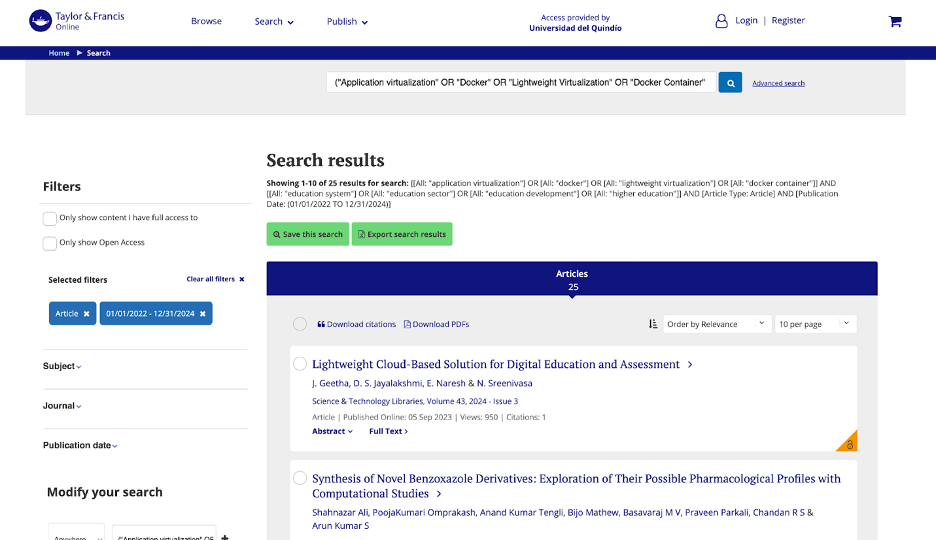
\includegraphics[width=\textwidth,keepaspectratio]{apendices/BD/criterios/TF-ed.png}
    \caption{Búsqueda de artículos de educación en Taylor \& Francis con criterios de inclusión/exclusión
    Fecha de acceso: 20/03/25 4:46 am
    }\label{fig:busqueda28}
\end{figure}
\FloatBarrier\begin{figure}[H]
    \centering
    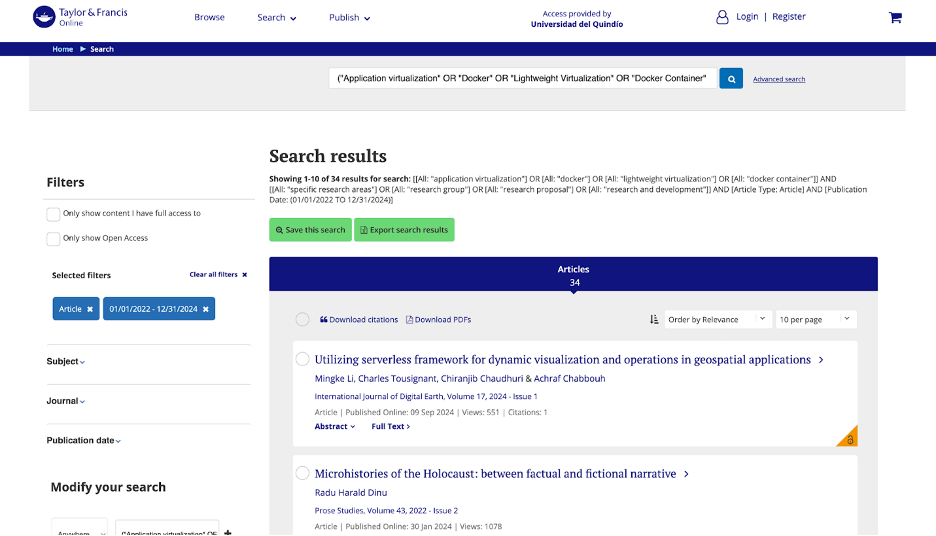
\includegraphics[width=\textwidth,keepaspectratio]{apendices/BD/criterios/TF-inv.png}
    \caption{Búsqueda de artículos de investigación en Taylor \& Francis con criterios de inclusión/exclusión
    Fecha de acceso: 20/03/25 4:49 am
    }\label{fig:busqueda29}
\end{figure}
\FloatBarrier\begin{figure}[H]
    \centering
    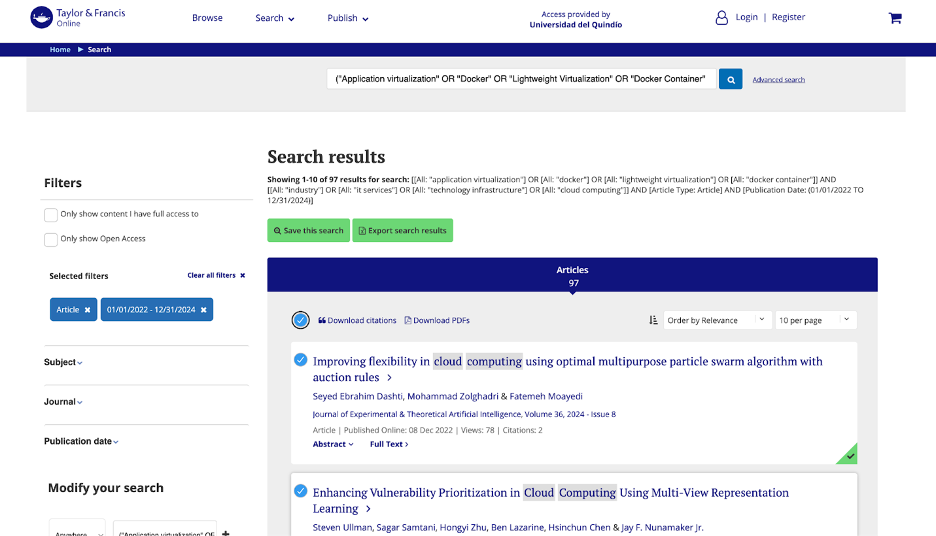
\includegraphics[width=\textwidth,keepaspectratio]{apendices/BD/criterios/TF-ind.png}
    \caption{Búsqueda de artículos de extensión en Taylor \& Francis con criterios de inclusión/exclusión
    Fecha de acceso: 20/03/25 4:50 am
    }\label{fig:busqueda30}
\end{figure}
\FloatBarrier\chapter{Plantilla del análisis DAR}
\section{Plantilla análisis DAR}

\begin{figure}[H]
    \centering
    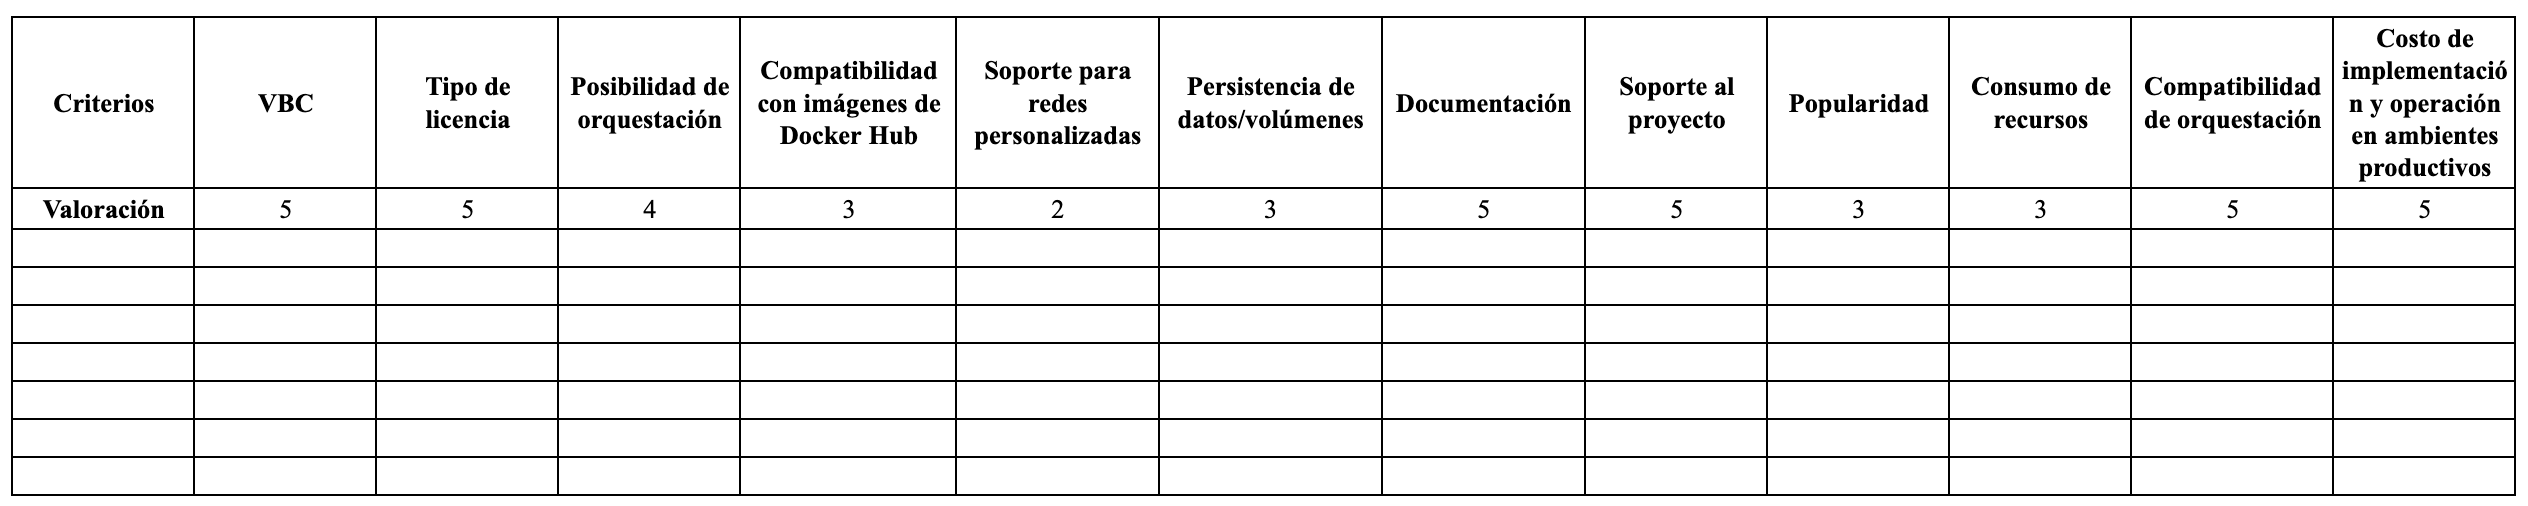
\includegraphics[width=\textwidth,height=0.85\textheight,keepaspectratio]{apendices/plantilla-DAR.png}
    \caption{Plantilla del análisis DAR}\label{fig:tabla-plantilla-dar}
\end{figure}
\FloatBarrier\chapter{Eventos de difusión}
\section{Seminario GRID 2024-II}


\section{Seminario GRID 2025-I}

\section{ACOFI 2025}

En esta sección se presenta la ponencia presentada en el congreso ACOFI 2025 como resultado de la investigación desarrollada en este trabajo.

\subsection{Páginas de la ponencia ACOFI}

% Página 1
\begin{figure}[H]
    \centering
    \begin{tcolorbox}[
        colback=white,
        colframe=gray!50,
        boxrule=1pt,
        arc=2pt,
        boxsep=5pt,
        left=3pt,
        right=3pt,
        top=3pt,
        bottom=3pt,
        drop shadow
    ]
        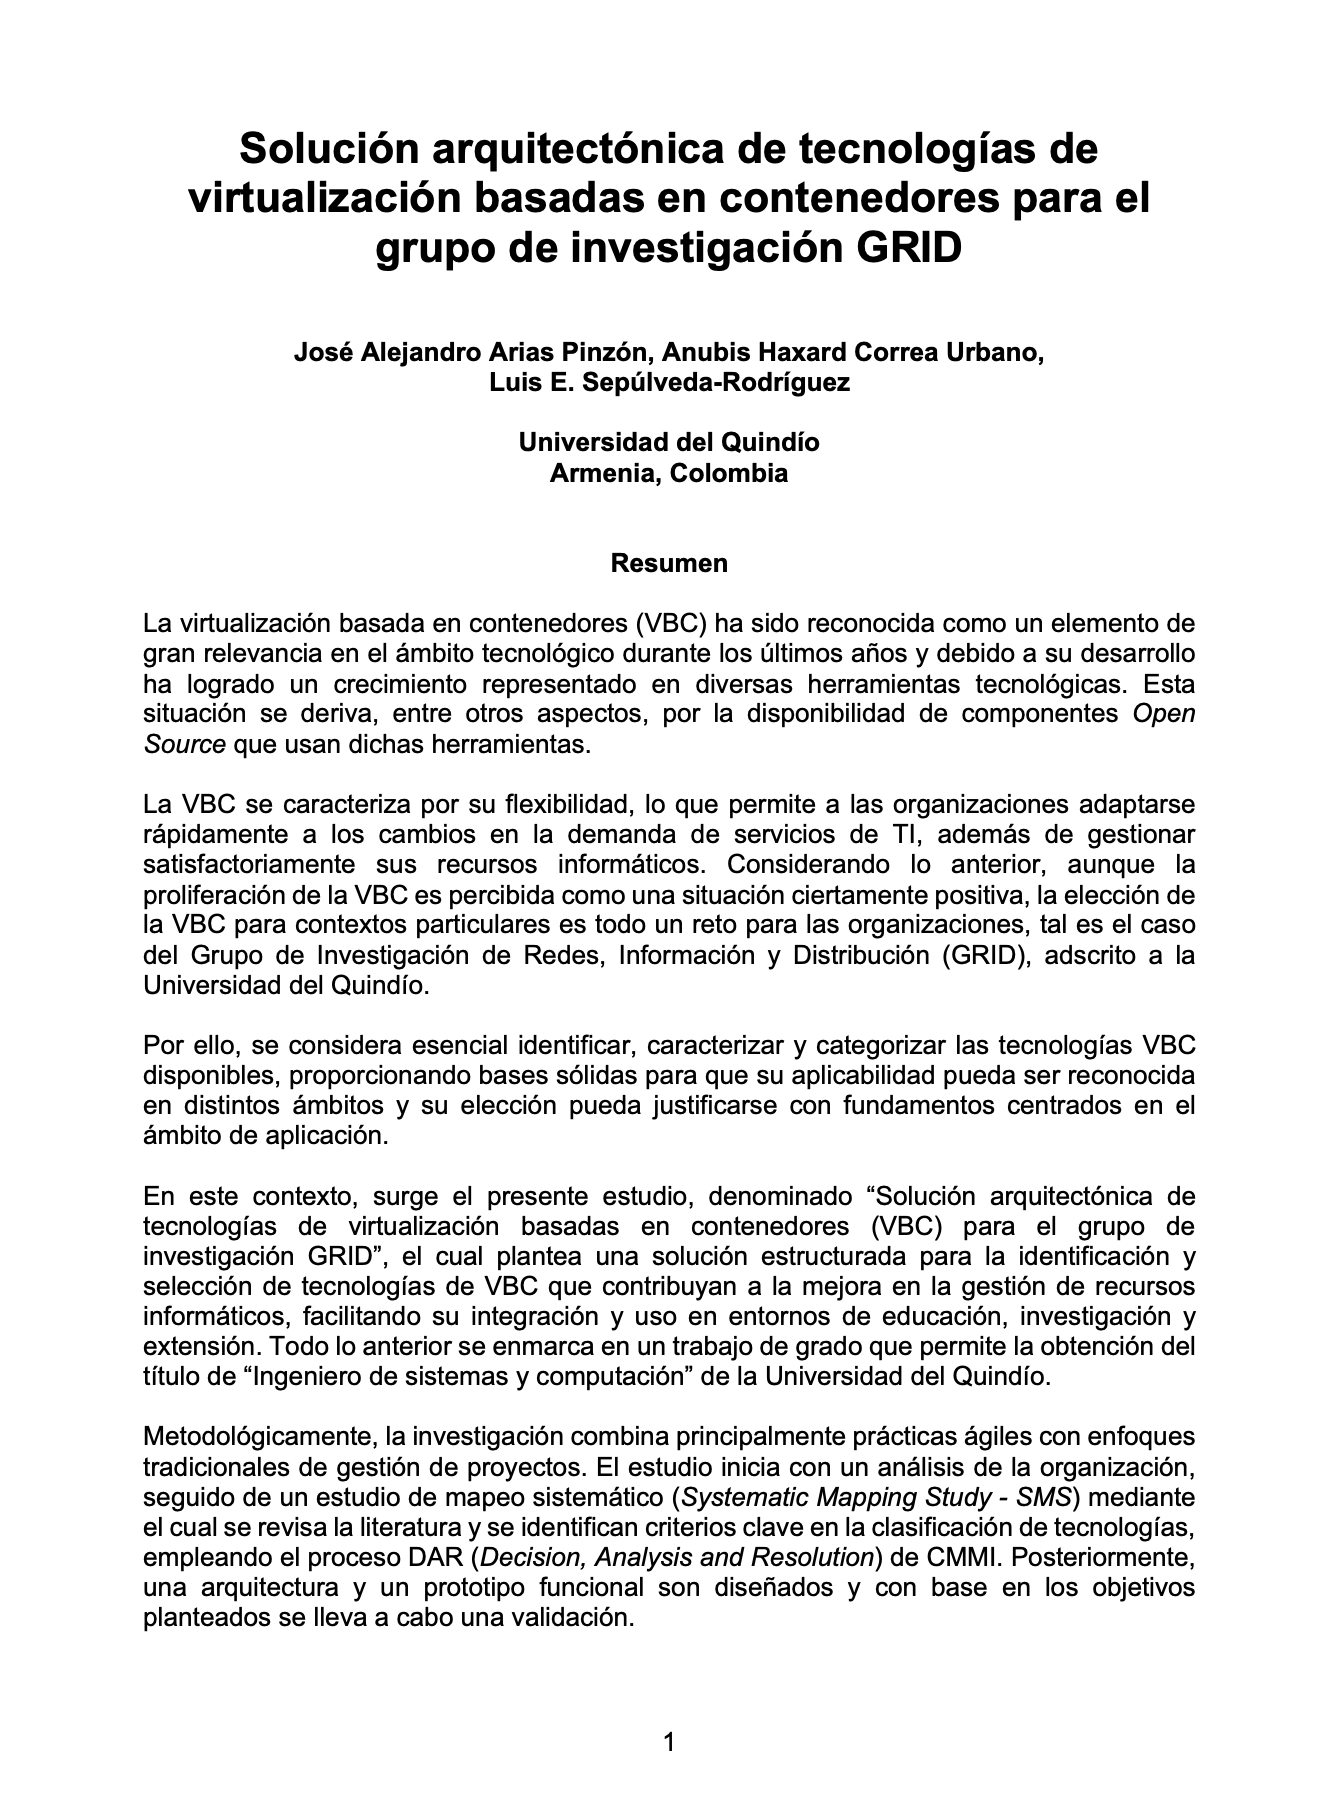
\includegraphics[width=0.95\textwidth,keepaspectratio]{apendices/ACOFI/pagina_1.png}
    \end{tcolorbox}
    \caption{Ponencia ACOFI --- Página 1}\label{fig:acofi-pagina-1}
\end{figure}
\FloatBarrier% Página 2
\begin{figure}[H]
    \centering
    \begin{tcolorbox}[
        colback=white,
        colframe=gray!50,
        boxrule=1pt,
        arc=2pt,
        boxsep=5pt,
        left=3pt,
        right=3pt,
        top=3pt,
        bottom=3pt,
        drop shadow
    ]
        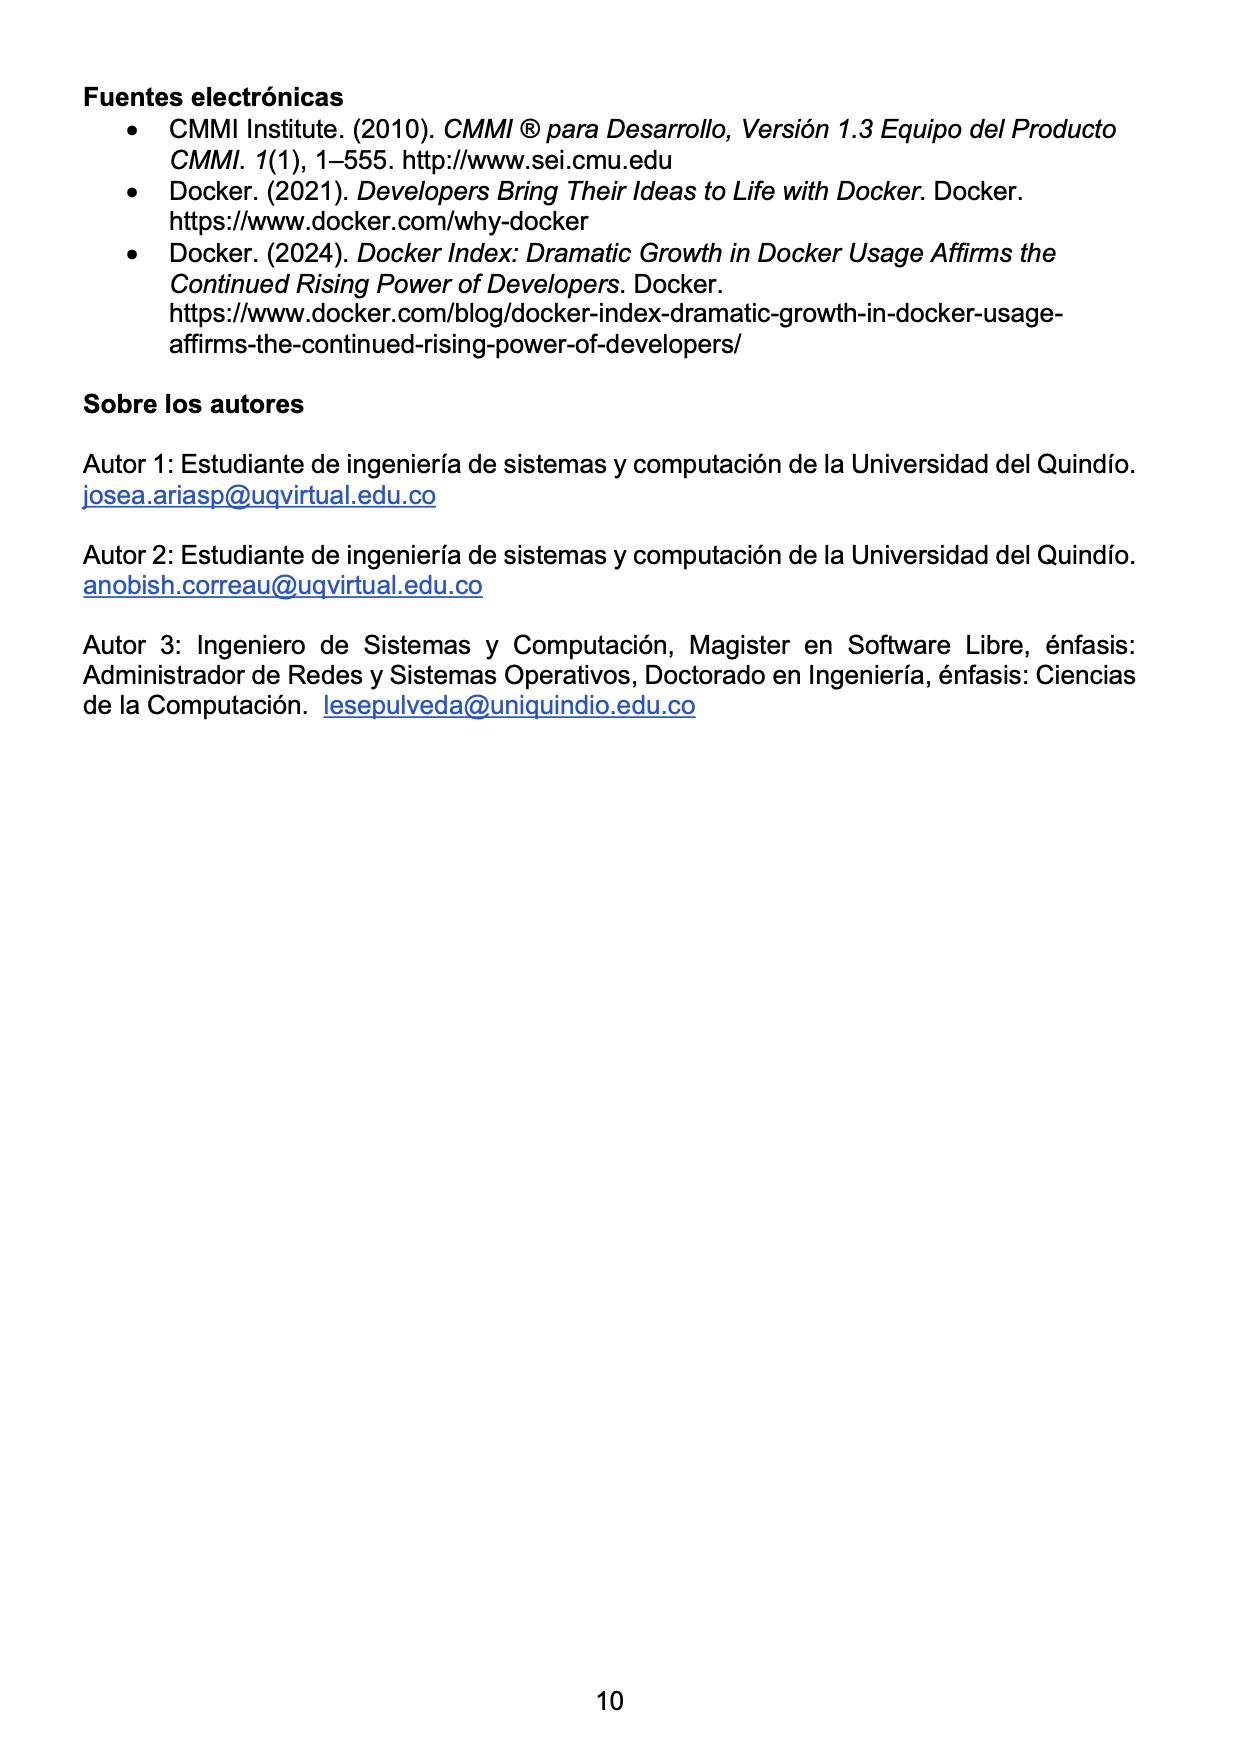
\includegraphics[width=0.95\textwidth,keepaspectratio]{apendices/ACOFI/pagina_2.png}
    \end{tcolorbox}
    \caption{Ponencia ACOFI --- Página 2}\label{fig:acofi-pagina-2}
\end{figure}
\FloatBarrier% Página 3
\begin{figure}[H]
    \centering
    \begin{tcolorbox}[
        colback=white,
        colframe=gray!50,
        boxrule=1pt,
        arc=2pt,
        boxsep=5pt,
        left=3pt,
        right=3pt,
        top=3pt,
        bottom=3pt,
        drop shadow
    ]
        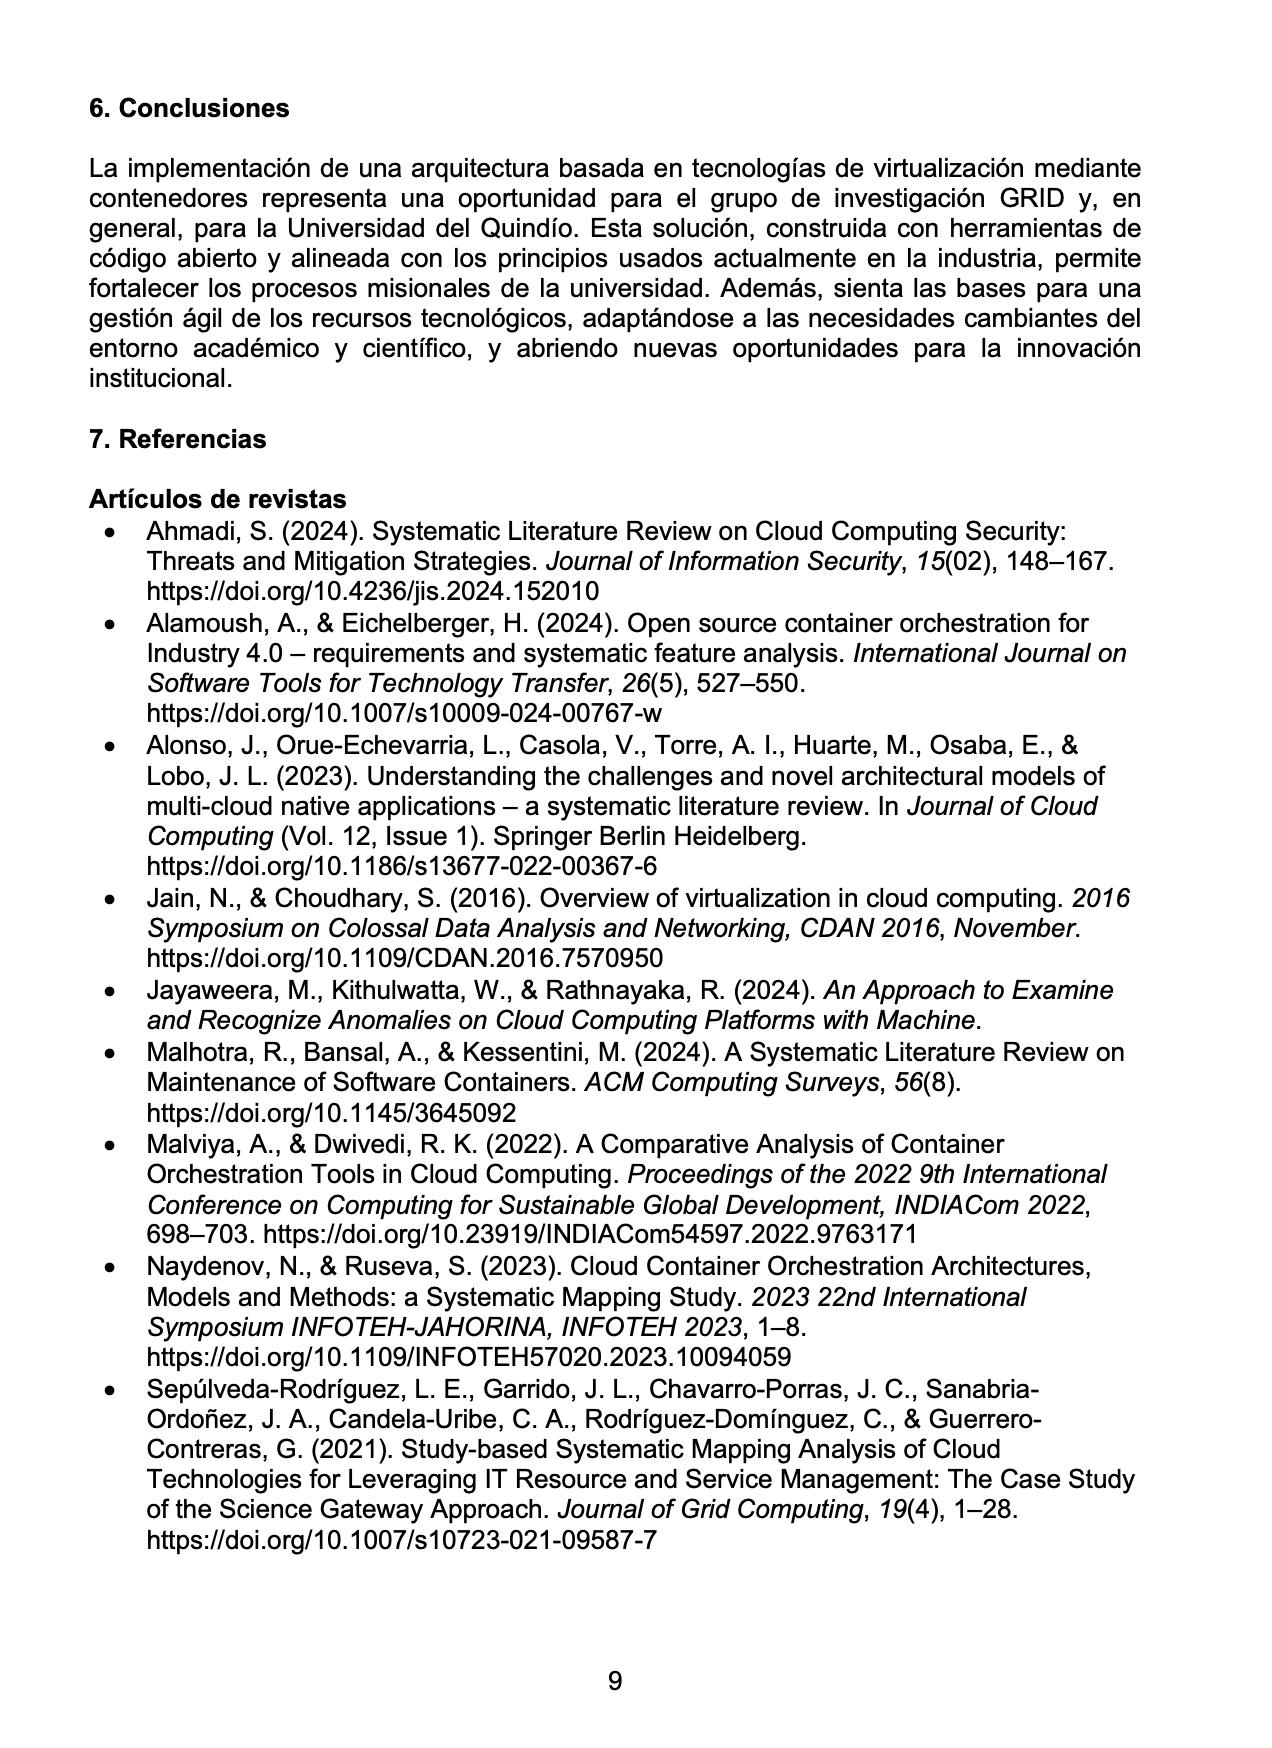
\includegraphics[width=0.95\textwidth,keepaspectratio]{apendices/ACOFI/pagina_3.png}
    \end{tcolorbox}
    \caption{Ponencia ACOFI --- Página 3}\label{fig:acofi-pagina-3}
\end{figure}
\FloatBarrier% Página 4
\begin{figure}[H]
    \centering
    \begin{tcolorbox}[
        colback=white,
        colframe=gray!50,
        boxrule=1pt,
        arc=2pt,
        boxsep=5pt,
        left=3pt,
        right=3pt,
        top=3pt,
        bottom=3pt,
        drop shadow
    ]
        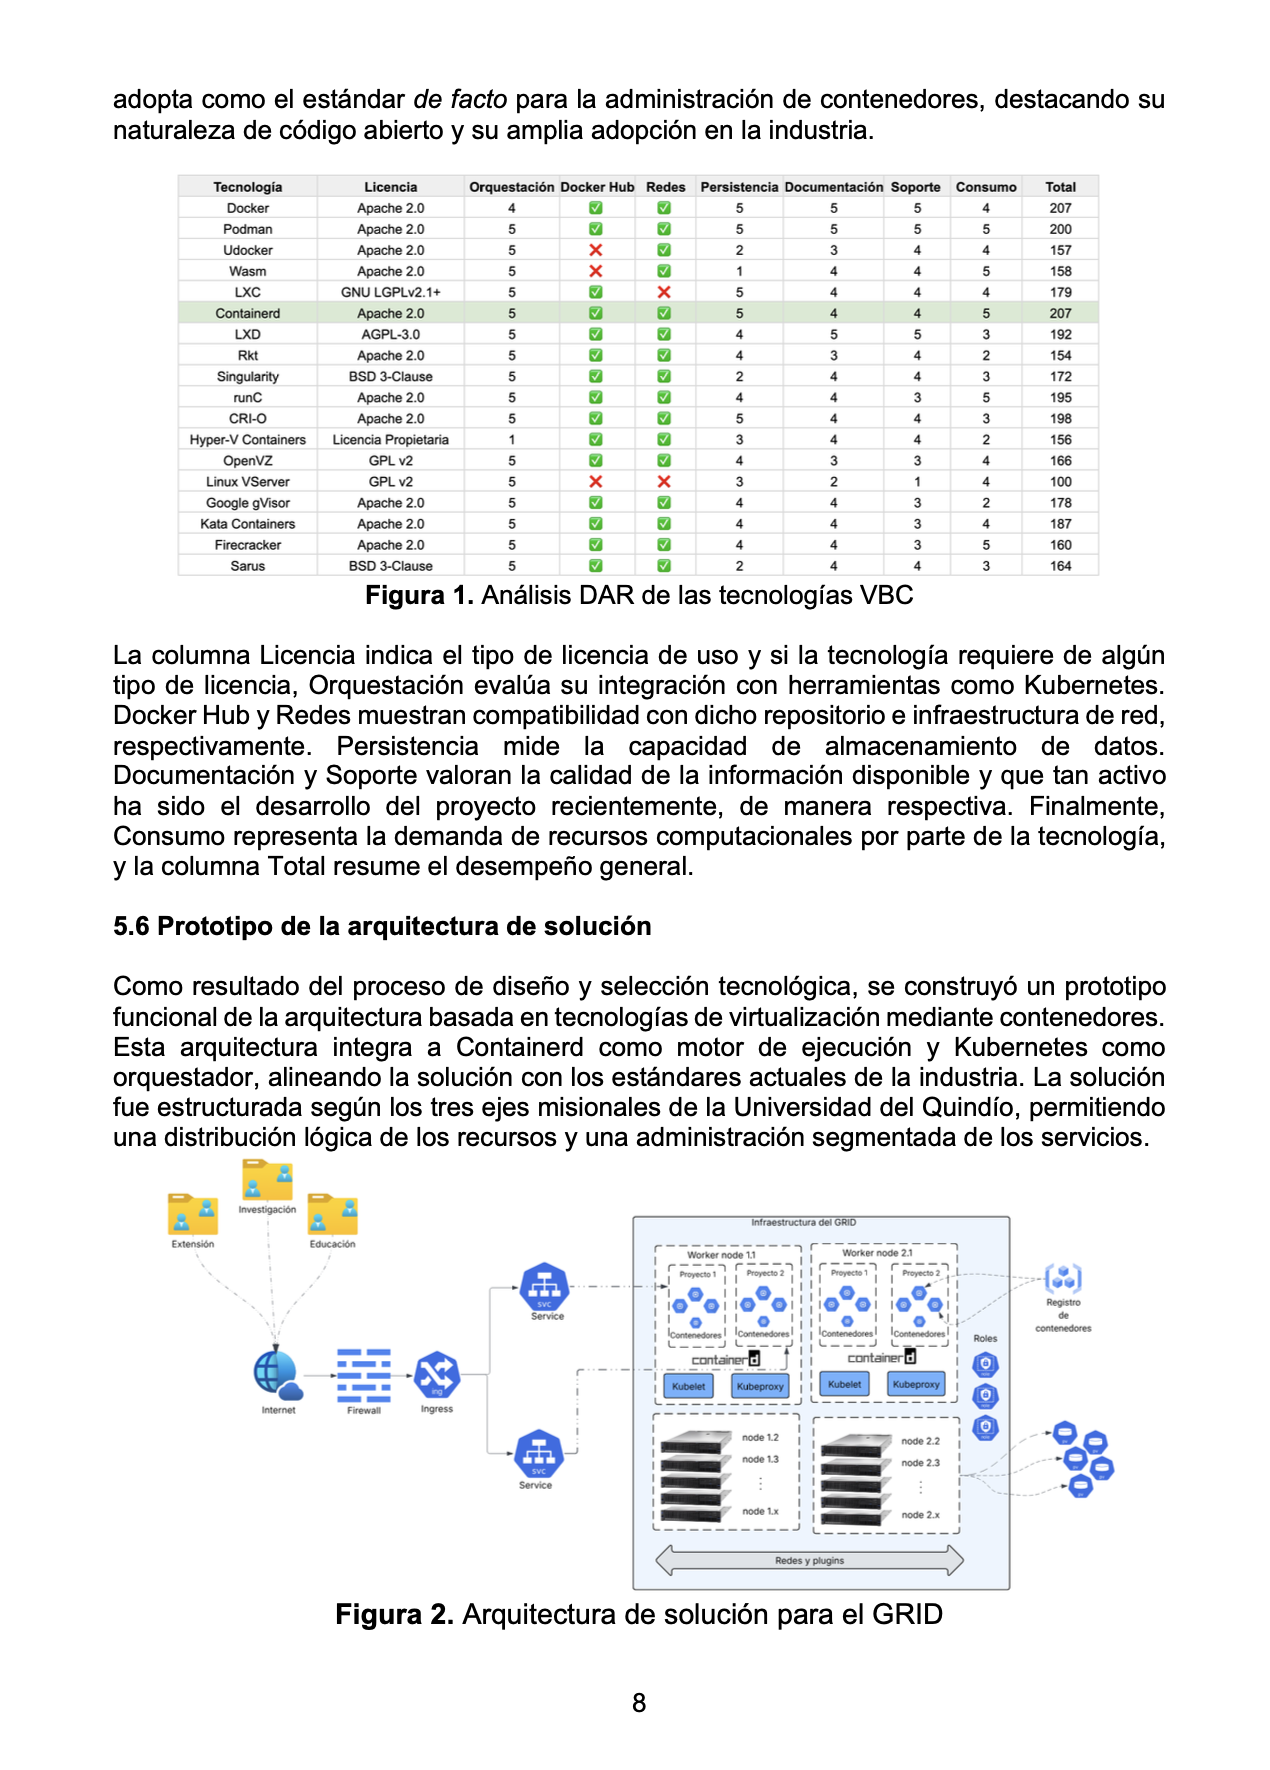
\includegraphics[width=0.95\textwidth,keepaspectratio]{apendices/ACOFI/pagina_4.png}
    \end{tcolorbox}
    \caption{Ponencia ACOFI --- Página 4}\label{fig:acofi-pagina-4}
\end{figure}
\FloatBarrier% Página 5
\begin{figure}[H]
    \centering
    \begin{tcolorbox}[
        colback=white,
        colframe=gray!50,
        boxrule=1pt,
        arc=2pt,
        boxsep=5pt,
        left=3pt,
        right=3pt,
        top=3pt,
        bottom=3pt,
        drop shadow
    ]
        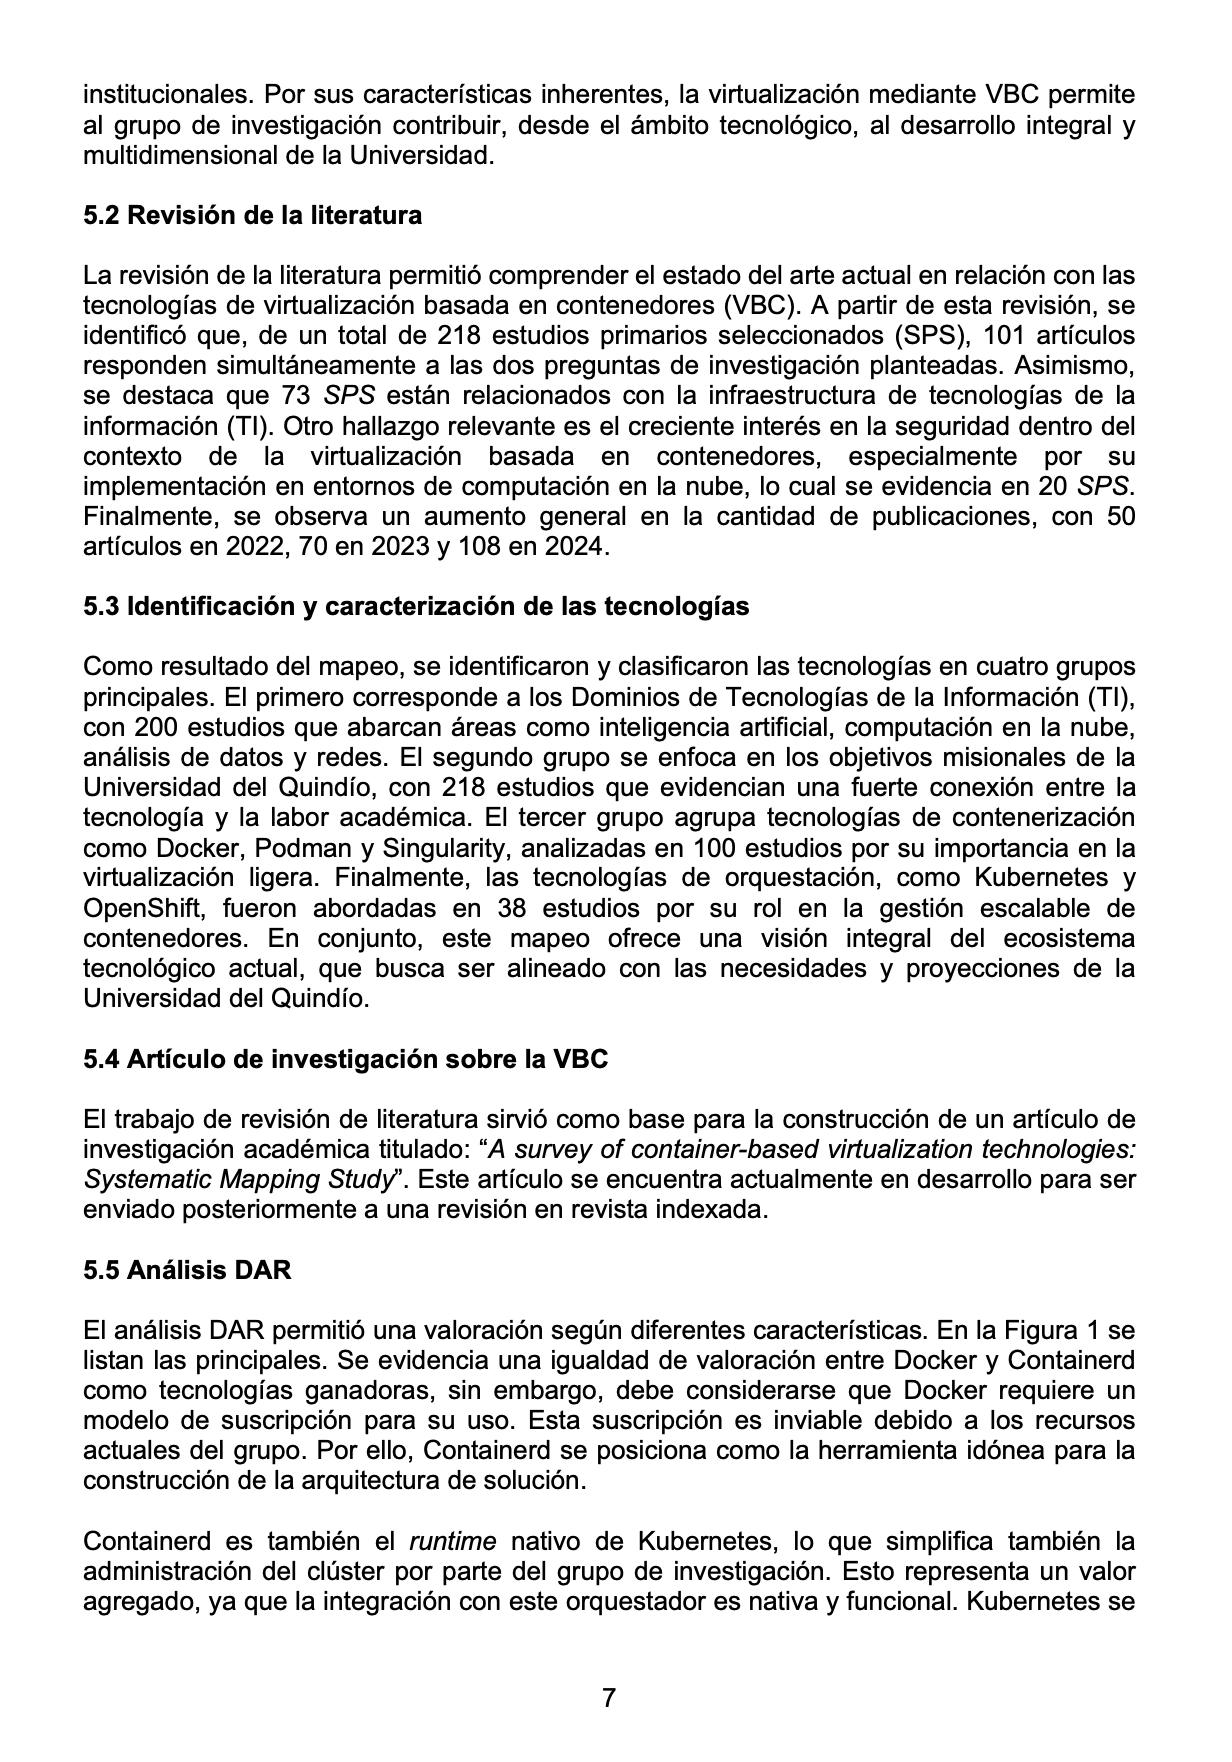
\includegraphics[width=0.95\textwidth,keepaspectratio]{apendices/ACOFI/pagina_5.png}
    \end{tcolorbox}
    \caption{Ponencia ACOFI --- Página 5}\label{fig:acofi-pagina-5}
\end{figure}
\FloatBarrier% Página 6
\begin{figure}[H]
    \centering
    \begin{tcolorbox}[
        colback=white,
        colframe=gray!50,
        boxrule=1pt,
        arc=2pt,
        boxsep=5pt,
        left=3pt,
        right=3pt,
        top=3pt,
        bottom=3pt,
        drop shadow
    ]
        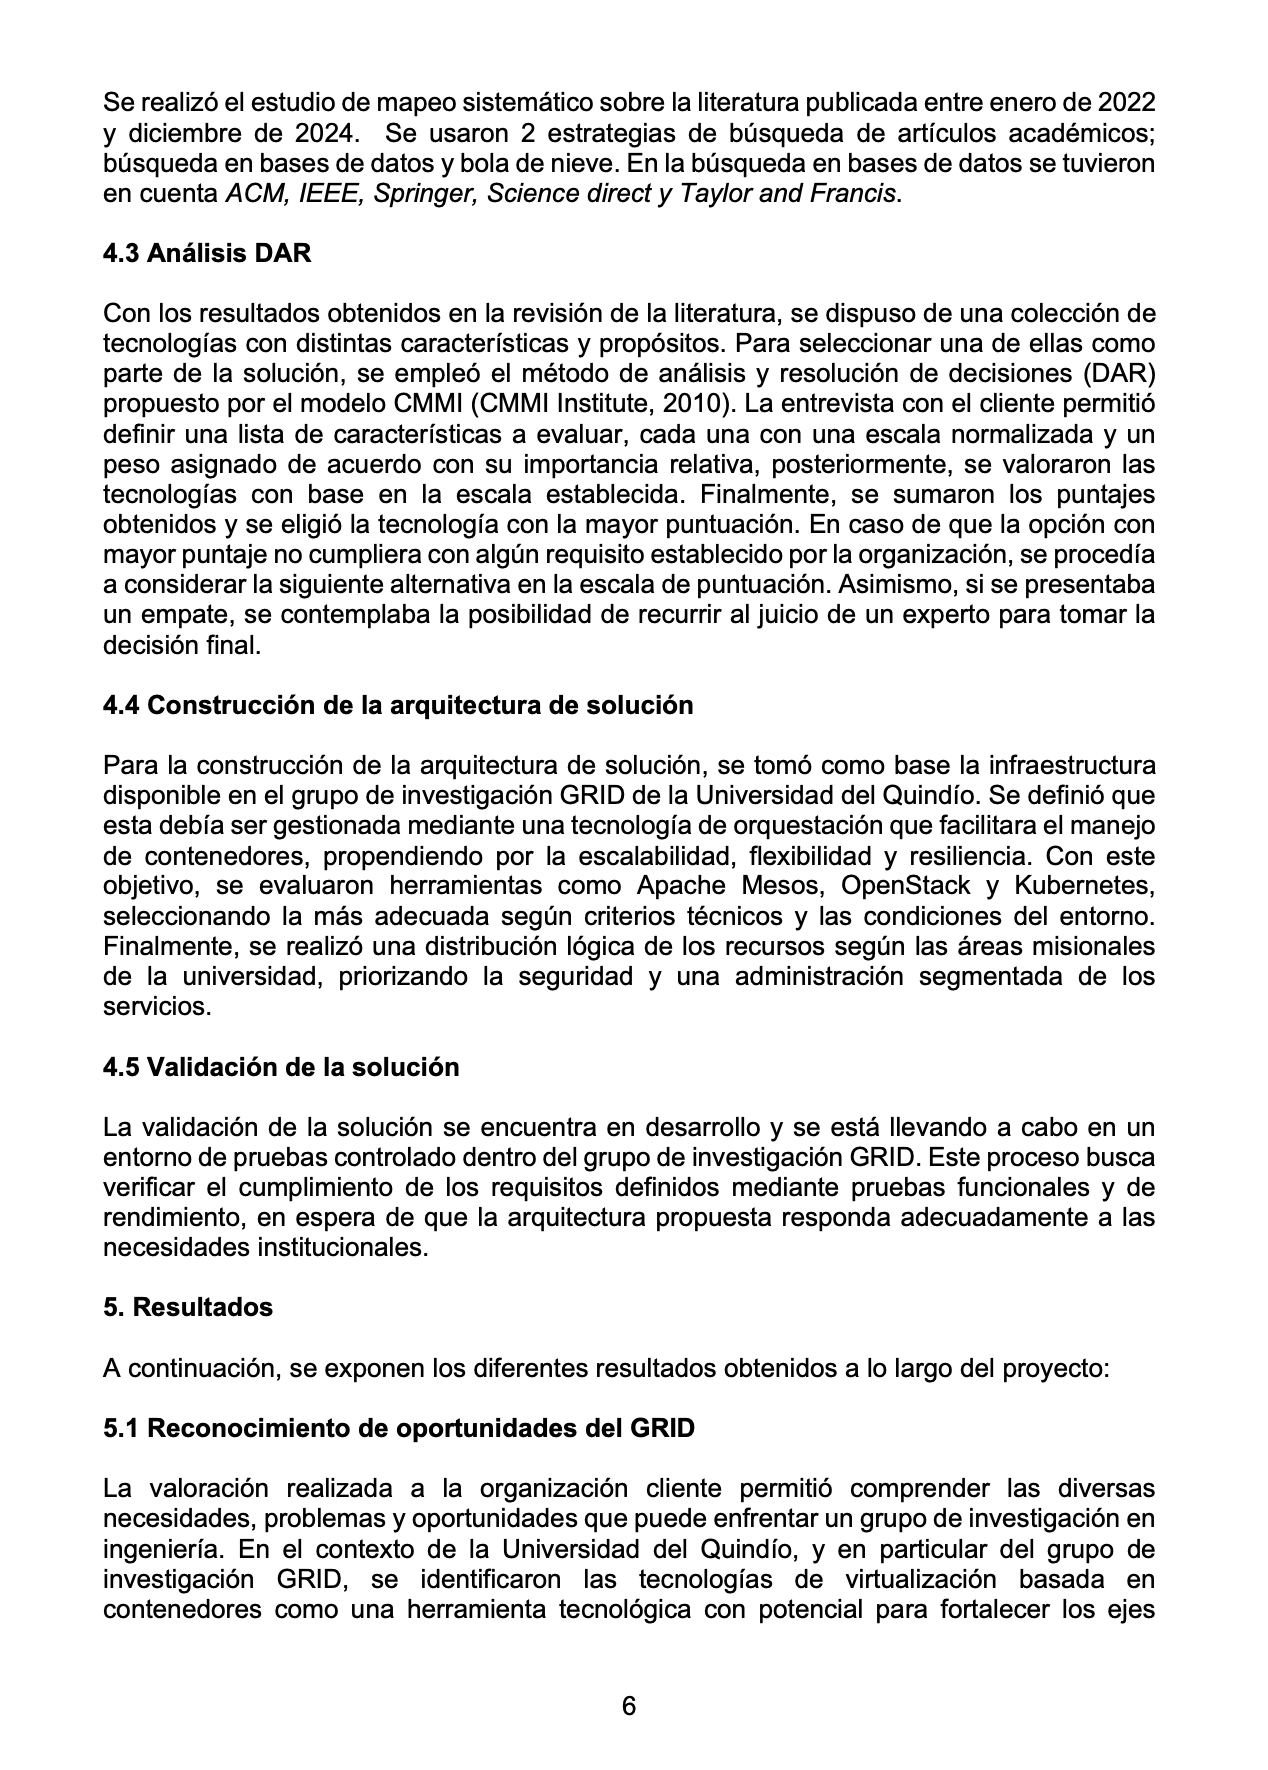
\includegraphics[width=0.95\textwidth,keepaspectratio]{apendices/ACOFI/pagina_6.png}
    \end{tcolorbox}
    \caption{Ponencia ACOFI --- Página 6}\label{fig:acofi-pagina-6}
\end{figure}
\FloatBarrier% Página 7
\begin{figure}[H]
    \centering
    \begin{tcolorbox}[
        colback=white,
        colframe=gray!50,
        boxrule=1pt,
        arc=2pt,
        boxsep=5pt,
        left=3pt,
        right=3pt,
        top=3pt,
        bottom=3pt,
        drop shadow
    ]
        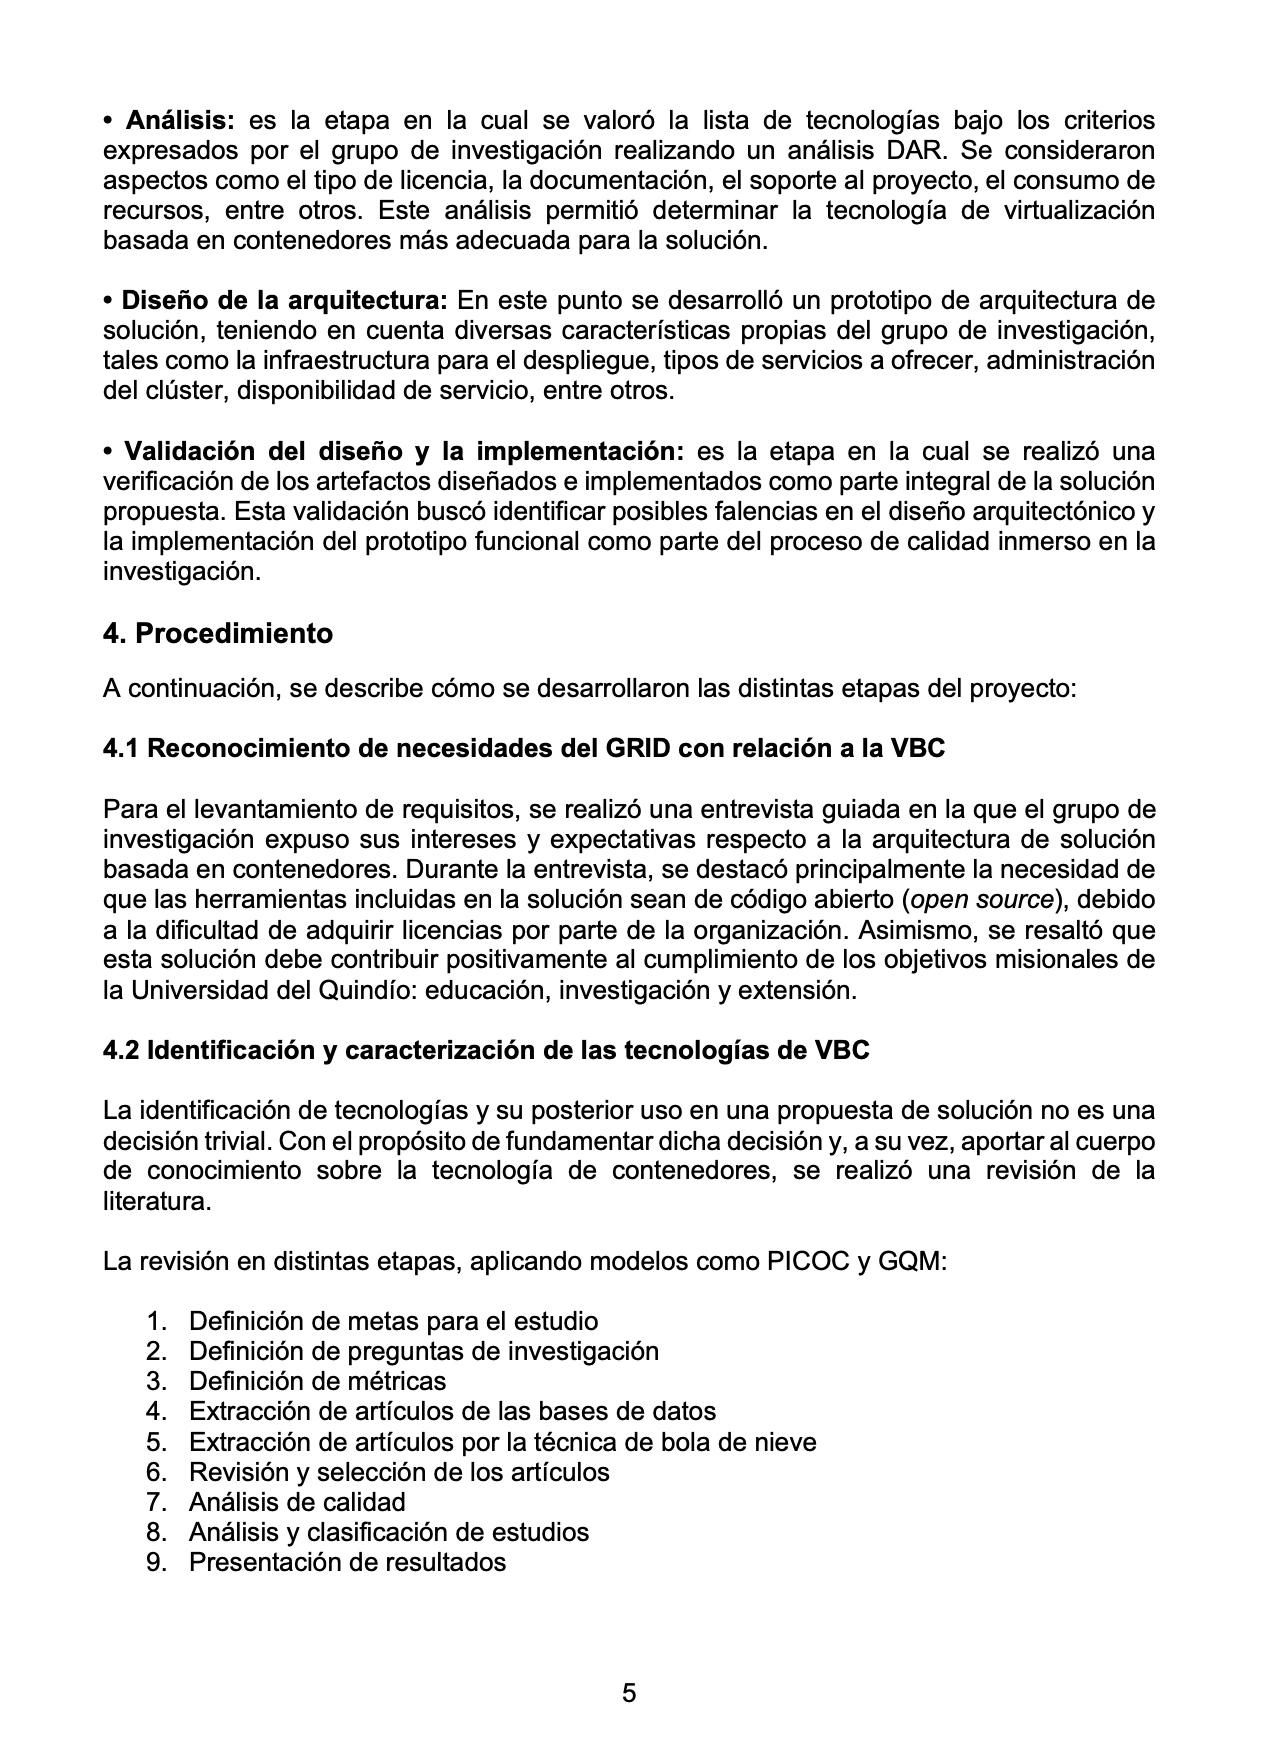
\includegraphics[width=0.95\textwidth,keepaspectratio]{apendices/ACOFI/pagina_7.png}
    \end{tcolorbox}
    \caption{Ponencia ACOFI --- Página 7}\label{fig:acofi-pagina-7}
\end{figure}
\FloatBarrier% Página 8
\begin{figure}[H]
    \centering
    \begin{tcolorbox}[
        colback=white,
        colframe=gray!50,
        boxrule=1pt,
        arc=2pt,
        boxsep=5pt,
        left=3pt,
        right=3pt,
        top=3pt,
        bottom=3pt,
        drop shadow
    ]
        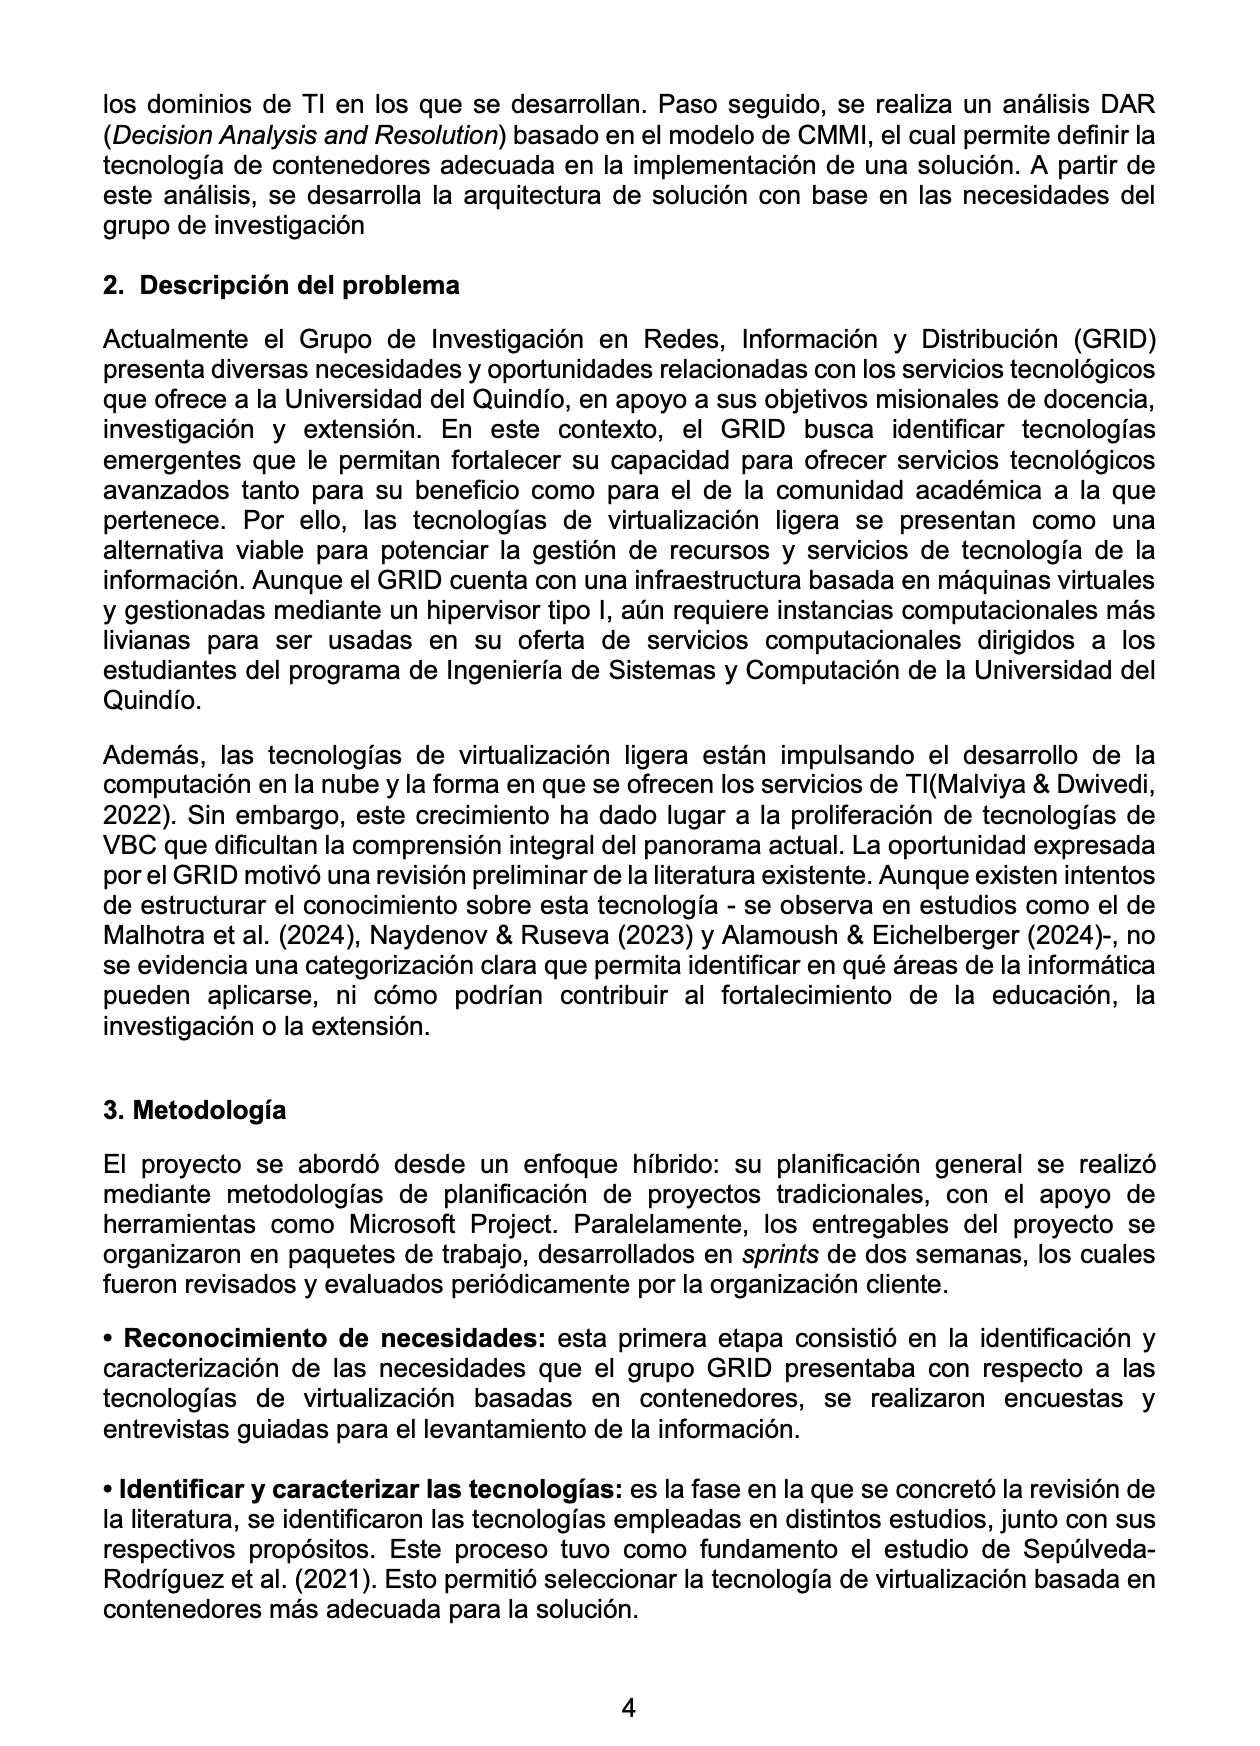
\includegraphics[width=0.95\textwidth,keepaspectratio]{apendices/ACOFI/pagina_8.png}
    \end{tcolorbox}
    \caption{Ponencia ACOFI --- Página 8}\label{fig:acofi-pagina-8}
\end{figure}
\FloatBarrier% Página 9
\begin{figure}[H]
    \centering
    \begin{tcolorbox}[
        colback=white,
        colframe=gray!50,
        boxrule=1pt,
        arc=2pt,
        boxsep=5pt,
        left=3pt,
        right=3pt,
        top=3pt,
        bottom=3pt,
        drop shadow
    ]
        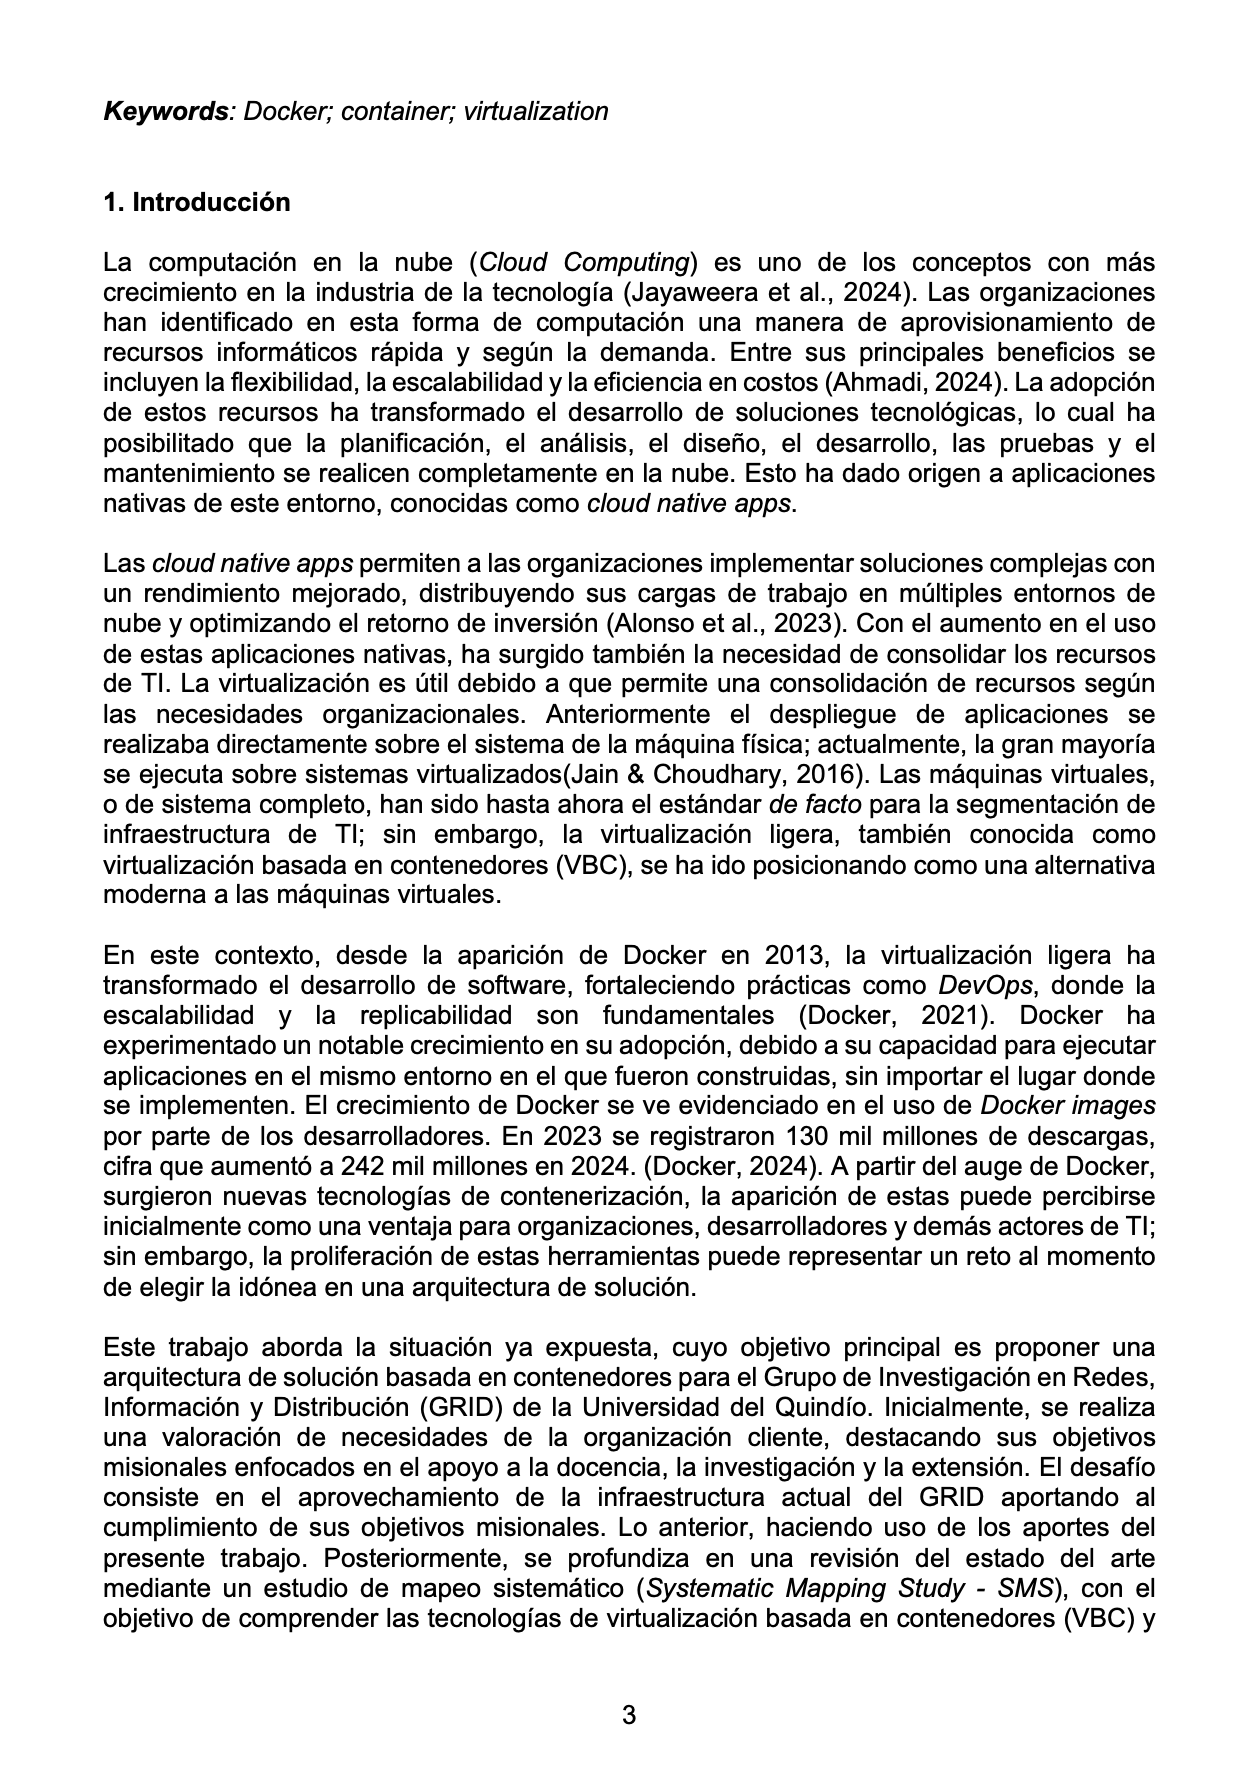
\includegraphics[width=0.95\textwidth,keepaspectratio]{apendices/ACOFI/pagina_9.png}
    \end{tcolorbox}
    \caption{Ponencia ACOFI --- Página 9}\label{fig:acofi-pagina-9}
\end{figure}
\FloatBarrier% Página 10
\begin{figure}[H]
    \centering
    \begin{tcolorbox}[
        colback=white,
        colframe=gray!50,
        boxrule=1pt,
        arc=2pt,
        boxsep=5pt,
        left=3pt,
        right=3pt,
        top=3pt,
        bottom=3pt,
        drop shadow
    ]
        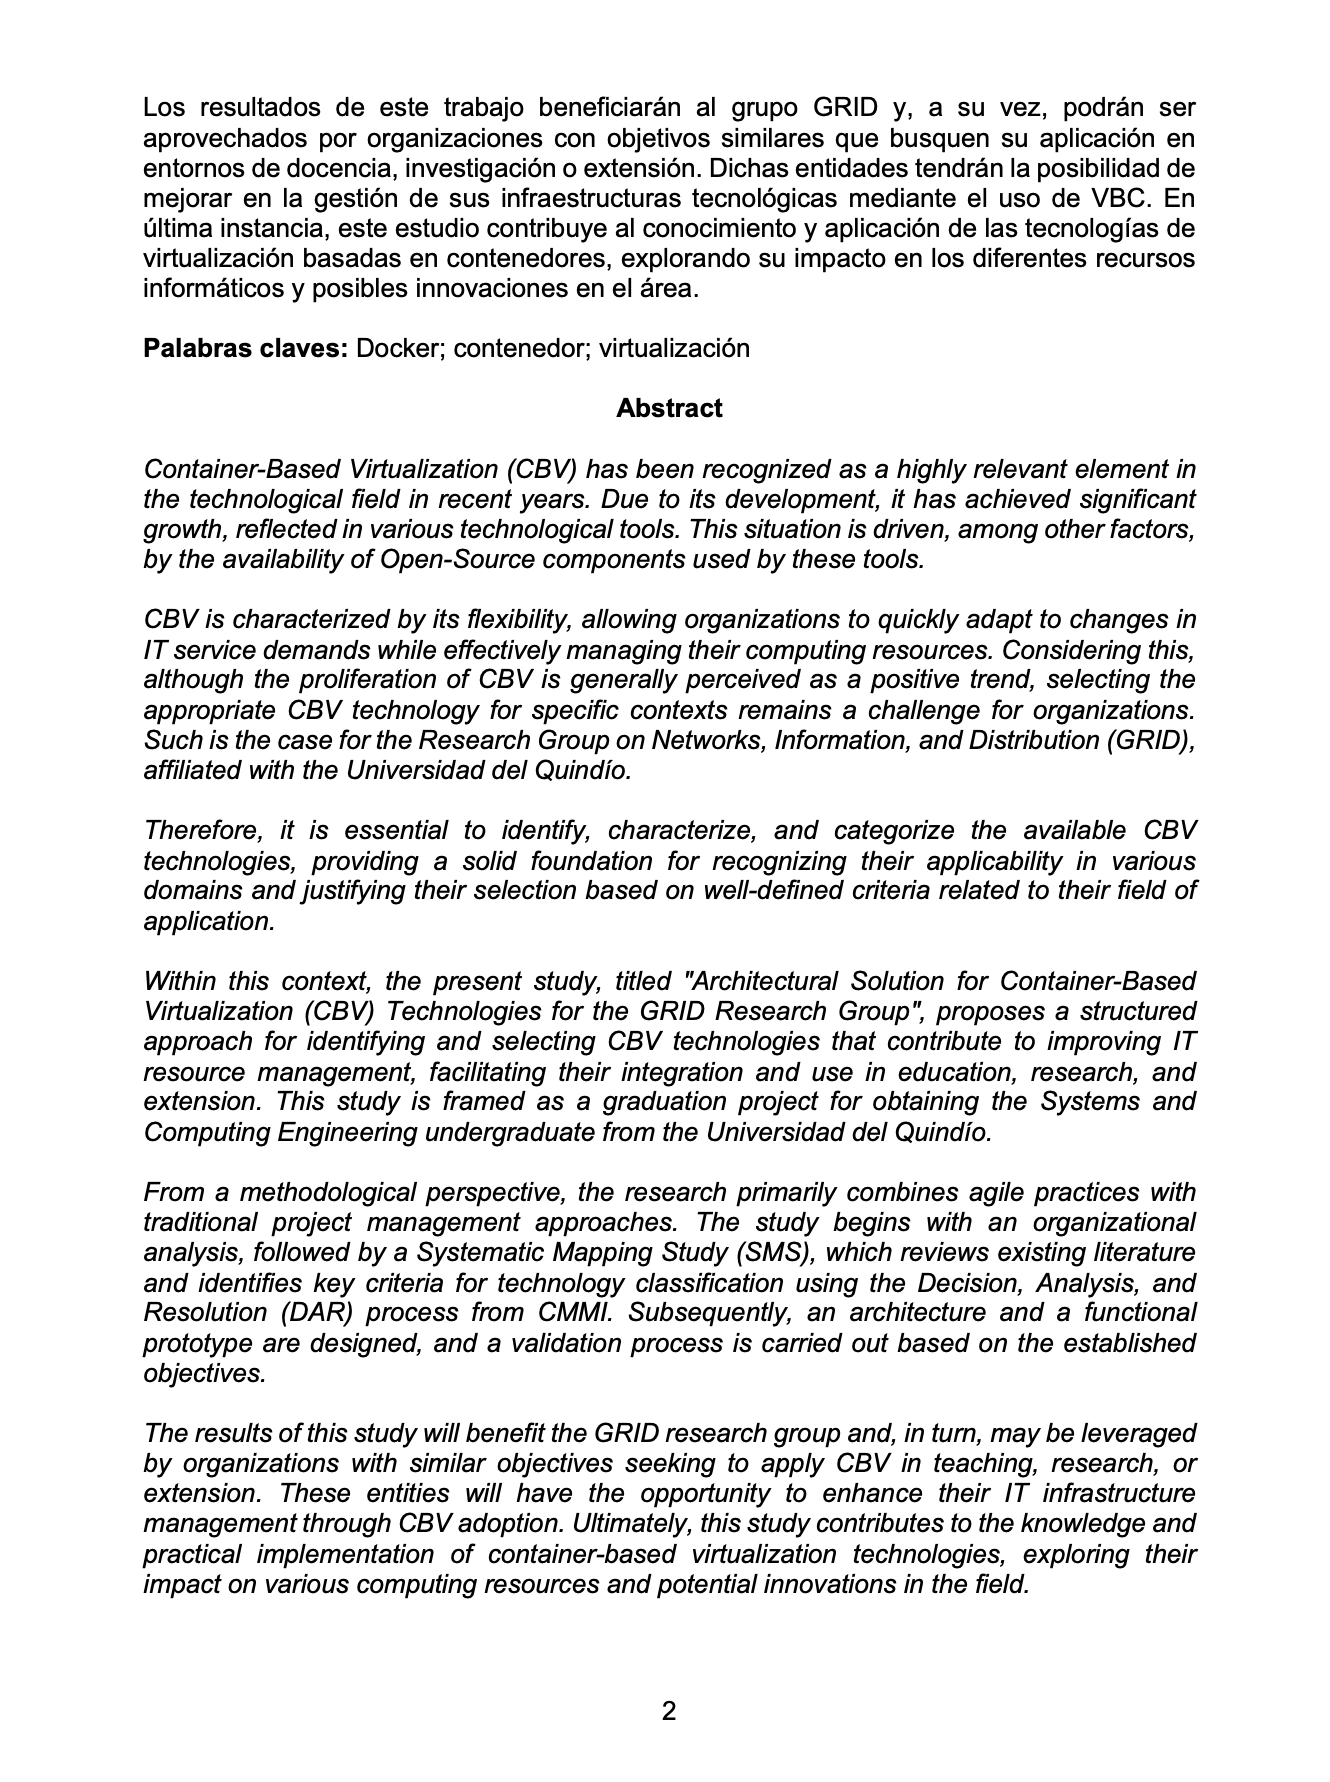
\includegraphics[width=0.95\textwidth,keepaspectratio]{apendices/ACOFI/pagina_10.png}
    \end{tcolorbox}
    \caption{Ponencia ACOFI --- Página 10}\label{fig:acofi-pagina-10}
\end{figure}
\FloatBarrier\section{CEIFI 2025}

\section{Artículo de revista}

En esta sección se presenta el artículo de revista publicado en Journal of Information Systems and Applications (JISA) como resultado de la investigación desarrollada en este trabajo.

\subsection{Páginas del artículo JISA}

% Página 1
\begin{figure}[H]
    \centering
    \begin{tcolorbox}[
        colback=white,
        colframe=gray!50,
        boxrule=1pt,
        arc=2pt,
        boxsep=5pt,
        left=3pt,
        right=3pt,
        top=3pt,
        bottom=3pt,
        drop shadow
    ]
        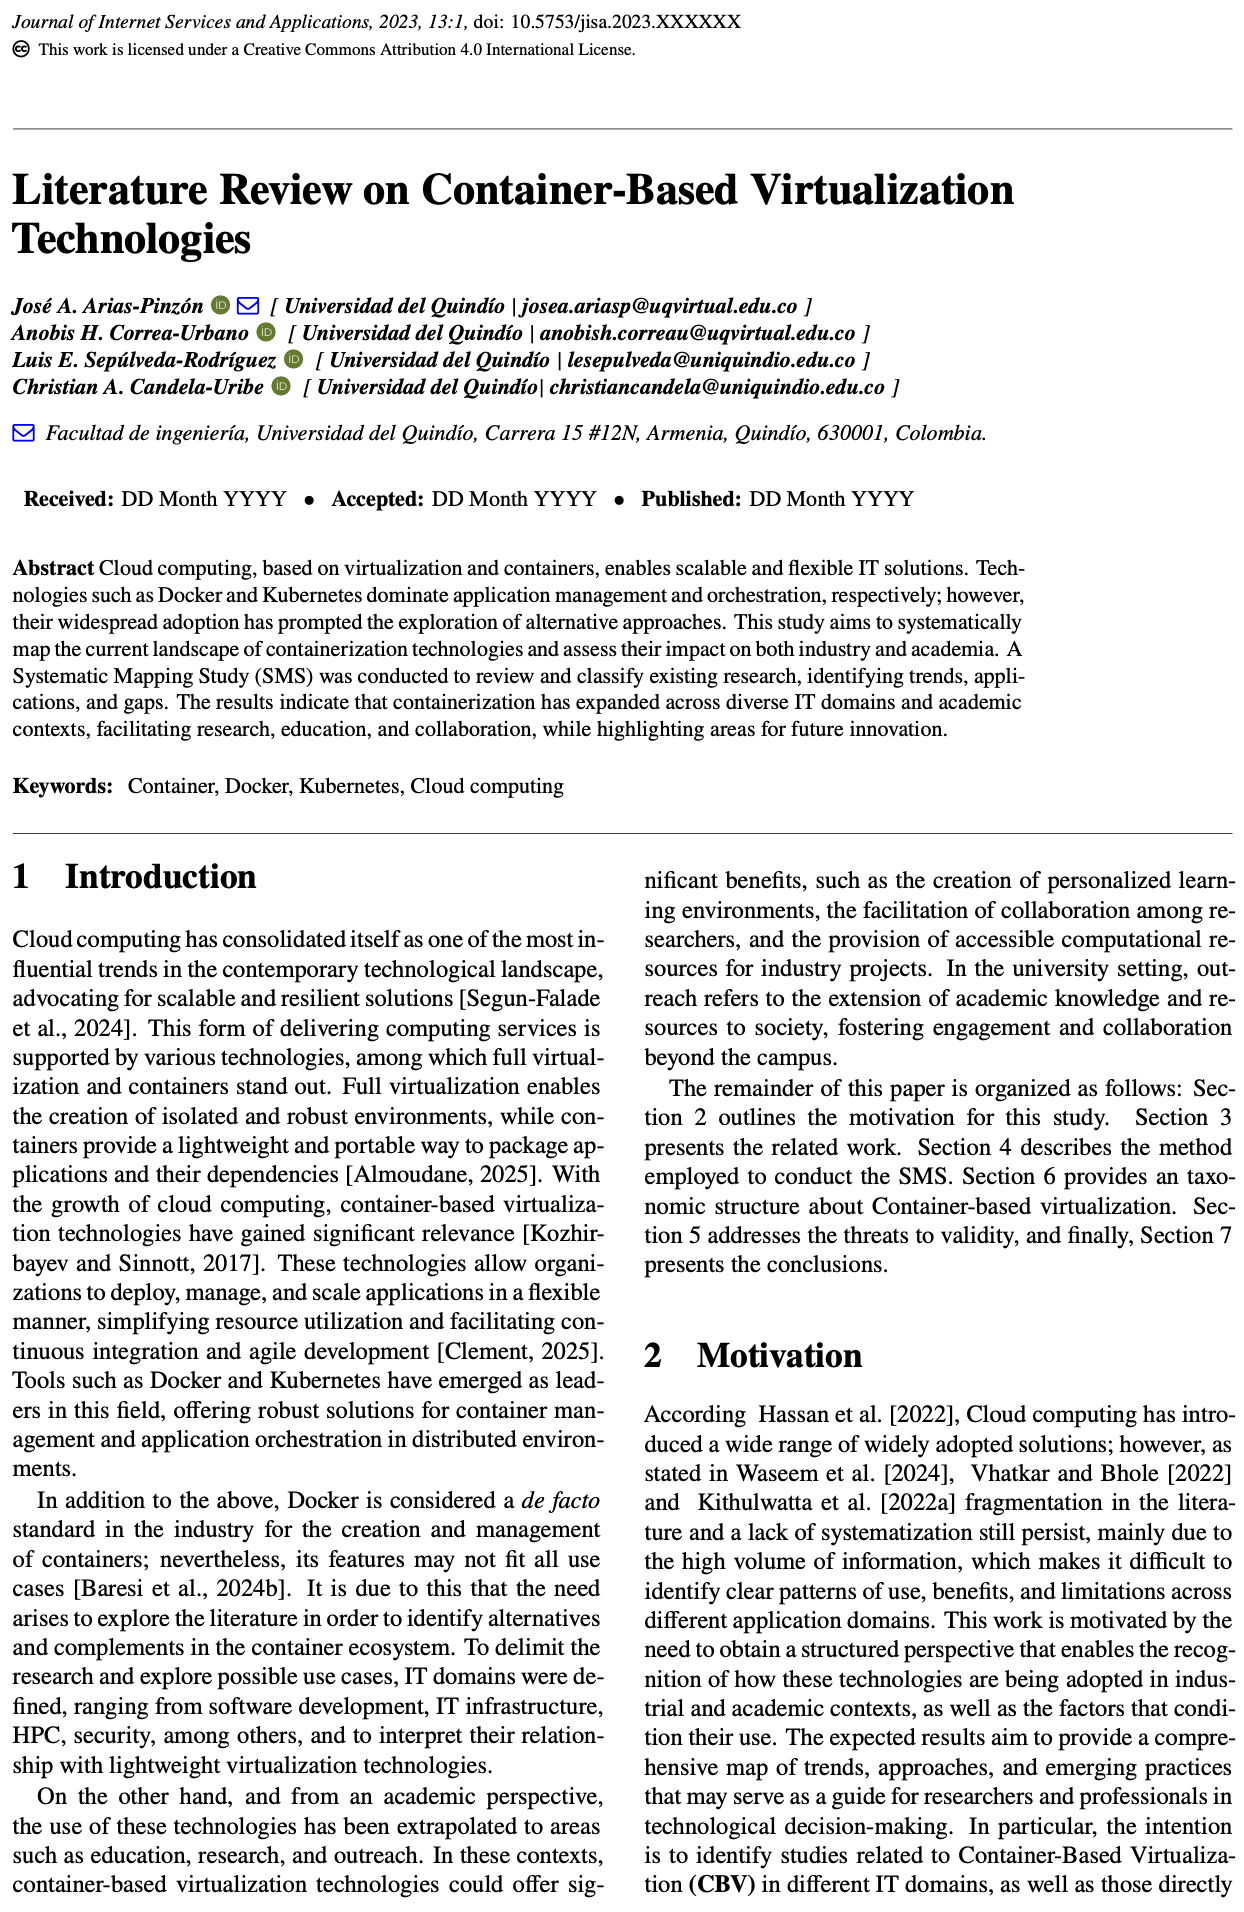
\includegraphics[width=0.95\textwidth,keepaspectratio]{apendices/JISA/pagina_1.png}
    \end{tcolorbox}
    \caption{Artículo JISA --- Página 1}\label{fig:jisa-pagina-1}
\end{figure}
\FloatBarrier% Página 2
\begin{figure}[H]
    \centering
    \begin{tcolorbox}[
        colback=white,
        colframe=gray!50,
        boxrule=1pt,
        arc=2pt,
        boxsep=5pt,
        left=3pt,
        right=3pt,
        top=3pt,
        bottom=3pt,
        drop shadow
    ]
        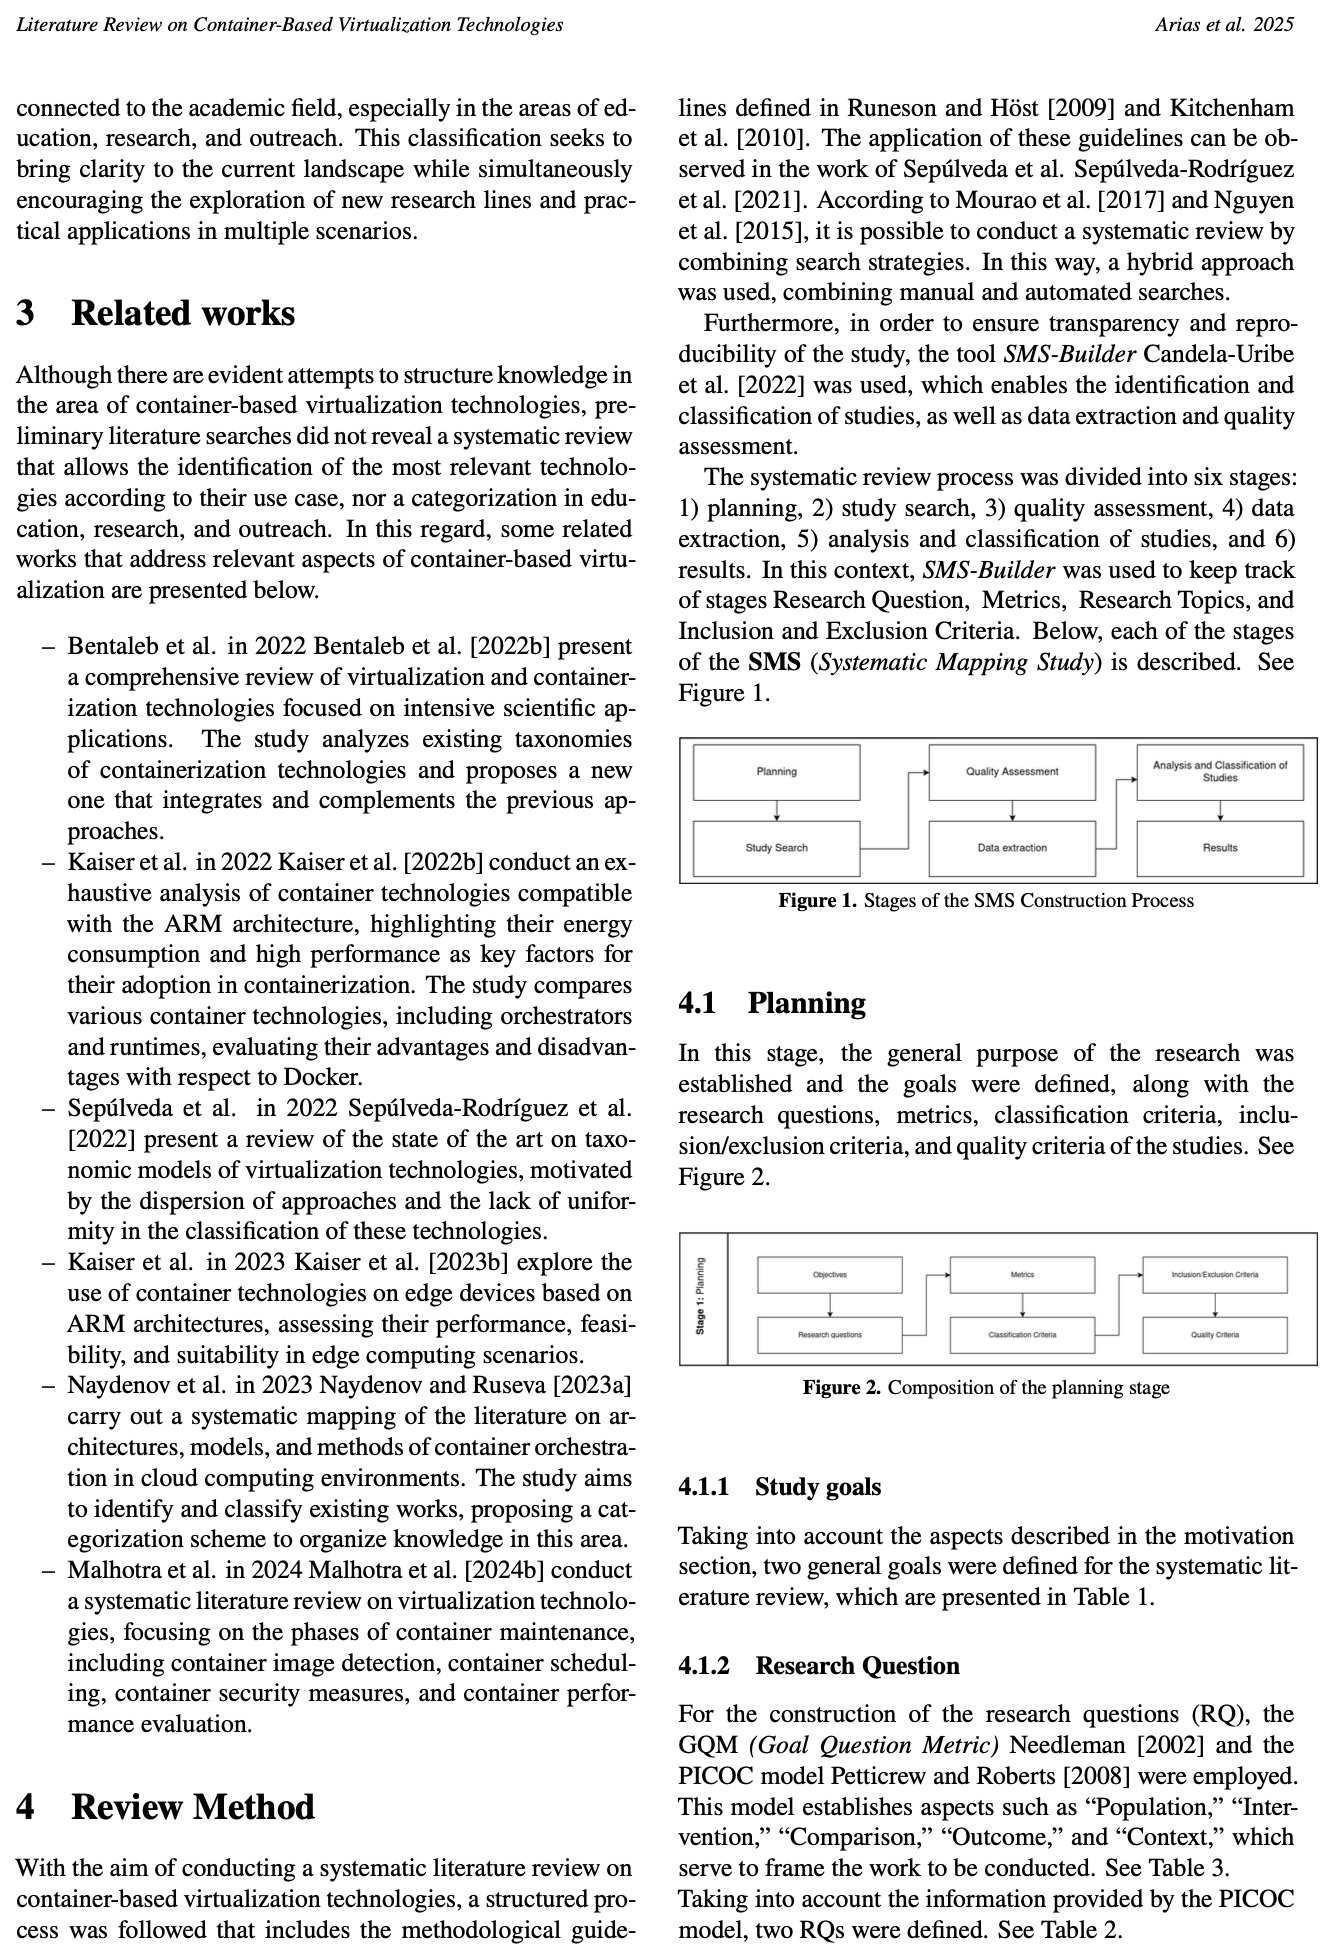
\includegraphics[width=0.95\textwidth,keepaspectratio]{apendices/JISA/pagina_2.png}
    \end{tcolorbox}
    \caption{Artículo JISA --- Página 2}\label{fig:jisa-pagina-2}
\end{figure}
\FloatBarrier% Página 3
\begin{figure}[H]
    \centering
    \begin{tcolorbox}[
        colback=white,
        colframe=gray!50,
        boxrule=1pt,
        arc=2pt,
        boxsep=5pt,
        left=3pt,
        right=3pt,
        top=3pt,
        bottom=3pt,
        drop shadow
    ]
        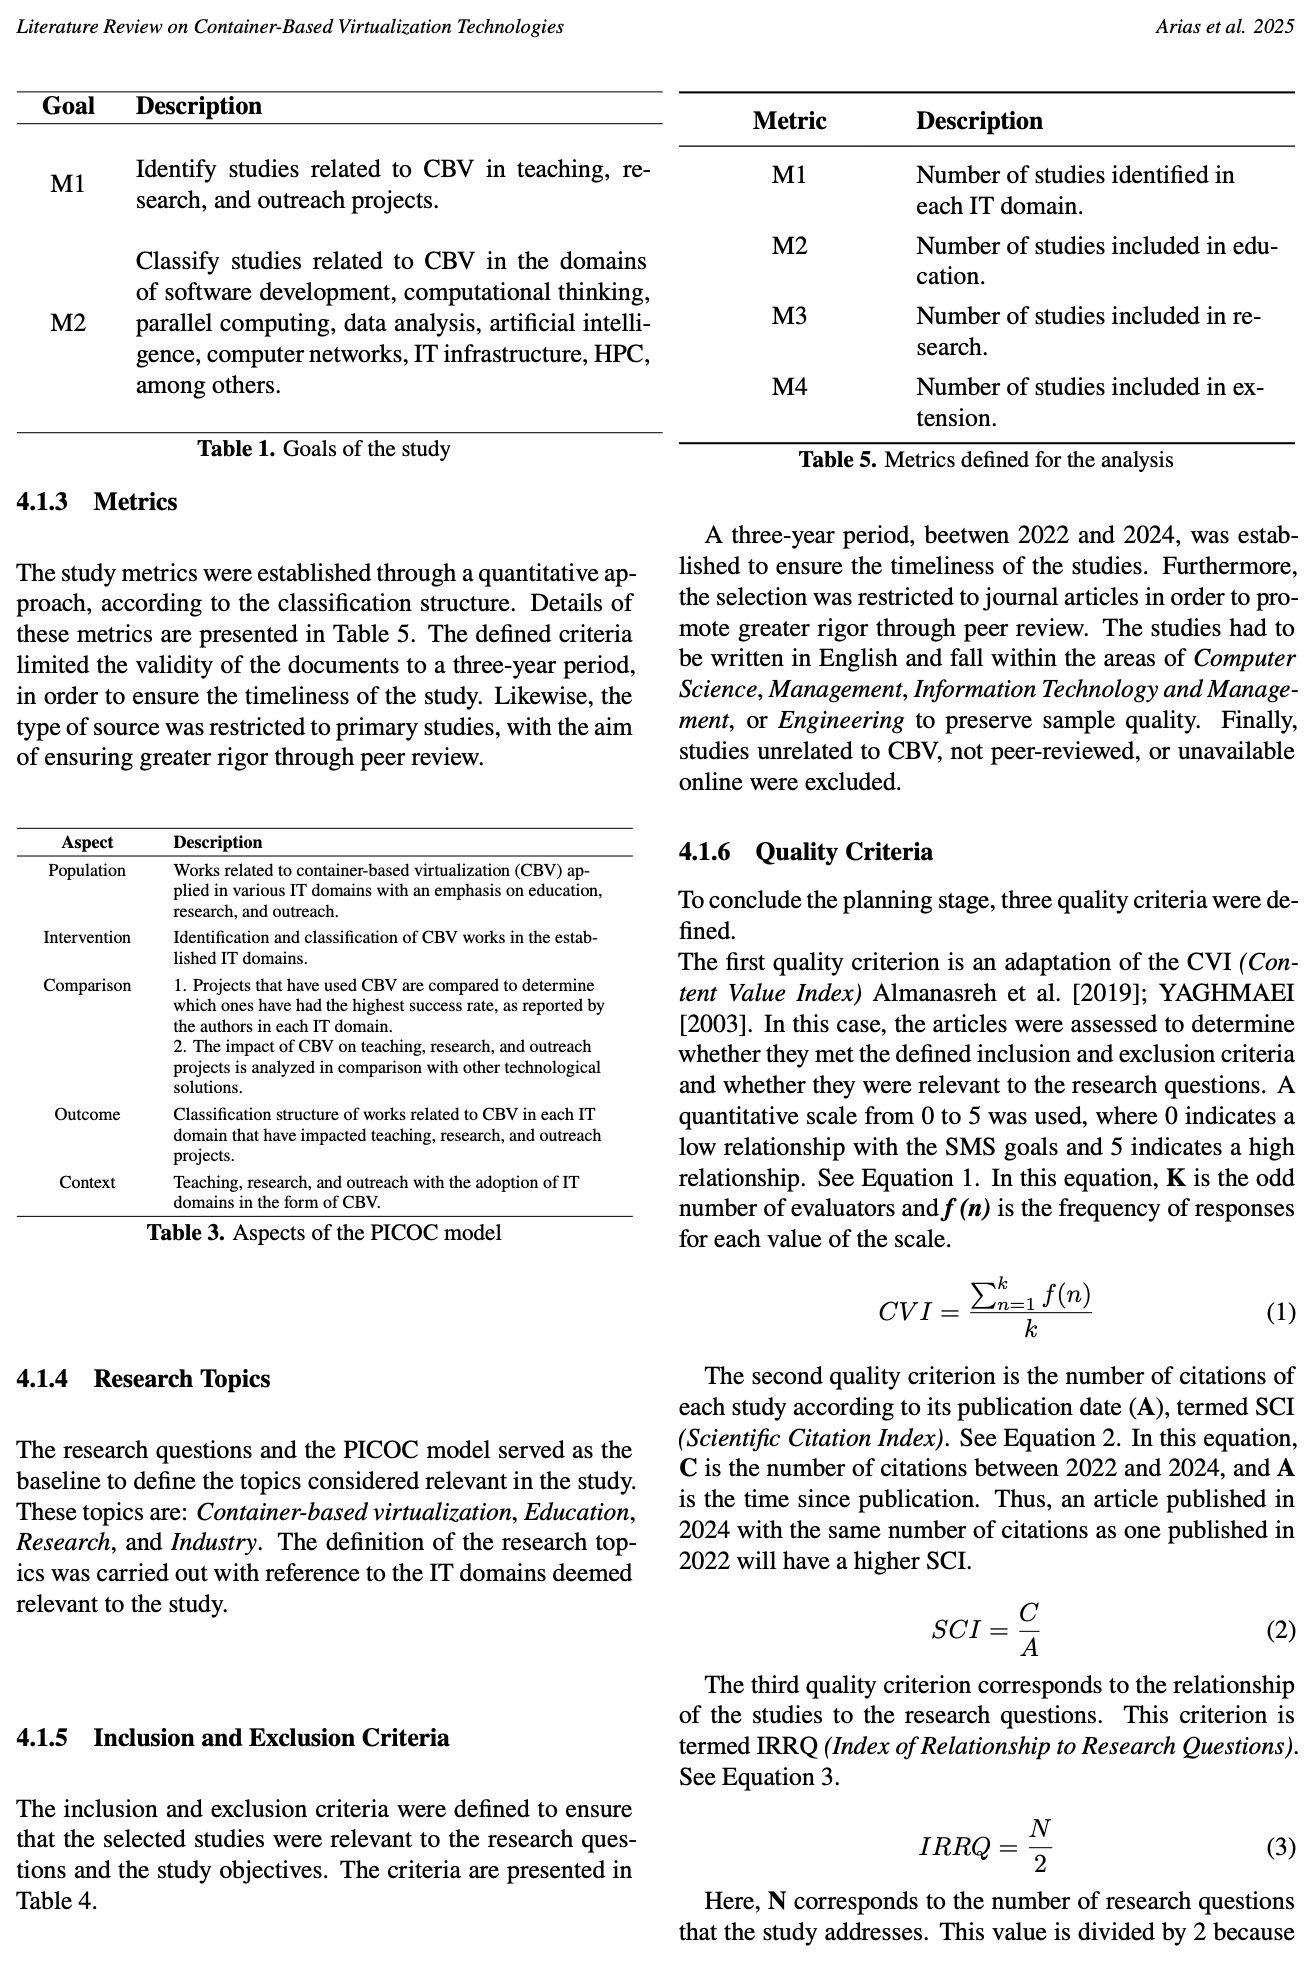
\includegraphics[width=0.95\textwidth,keepaspectratio]{apendices/JISA/pagina_3.png}
    \end{tcolorbox}
    \caption{Artículo JISA --- Página 3}\label{fig:jisa-pagina-3}
\end{figure}
\FloatBarrier% Página 4
\begin{figure}[H]
    \centering
    \begin{tcolorbox}[
        colback=white,
        colframe=gray!50,
        boxrule=1pt,
        arc=2pt,
        boxsep=5pt,
        left=3pt,
        right=3pt,
        top=3pt,
        bottom=3pt,
        drop shadow
    ]
        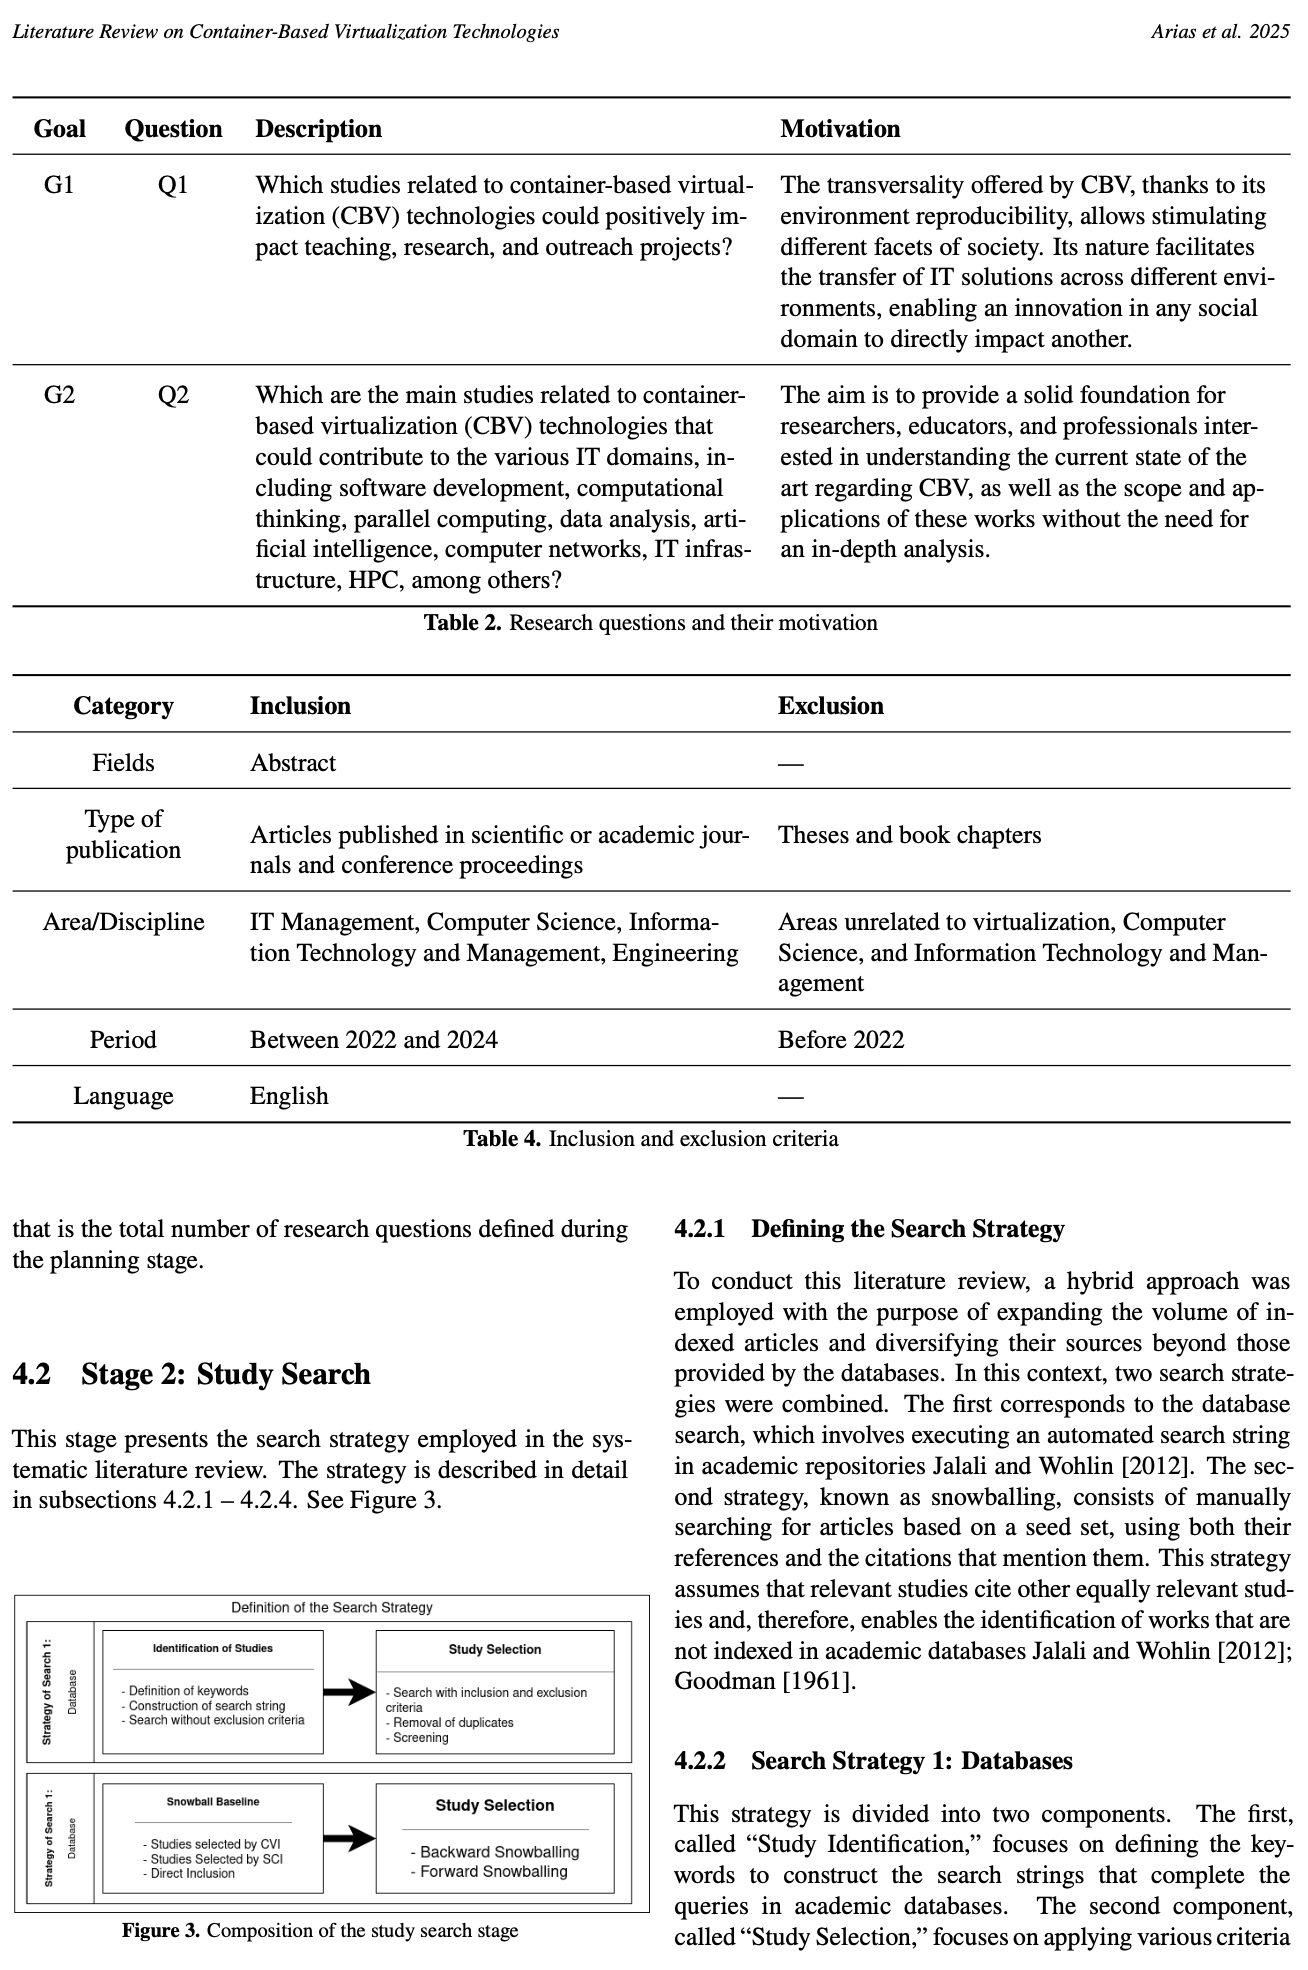
\includegraphics[width=0.95\textwidth,keepaspectratio]{apendices/JISA/pagina_4.png}
    \end{tcolorbox}
    \caption{Artículo JISA --- Página 4}\label{fig:jisa-pagina-4}
\end{figure}
\FloatBarrier% Página 5
\begin{figure}[H]
    \centering
    \begin{tcolorbox}[
        colback=white,
        colframe=gray!50,
        boxrule=1pt,
        arc=2pt,
        boxsep=5pt,
        left=3pt,
        right=3pt,
        top=3pt,
        bottom=3pt,
        drop shadow
    ]
        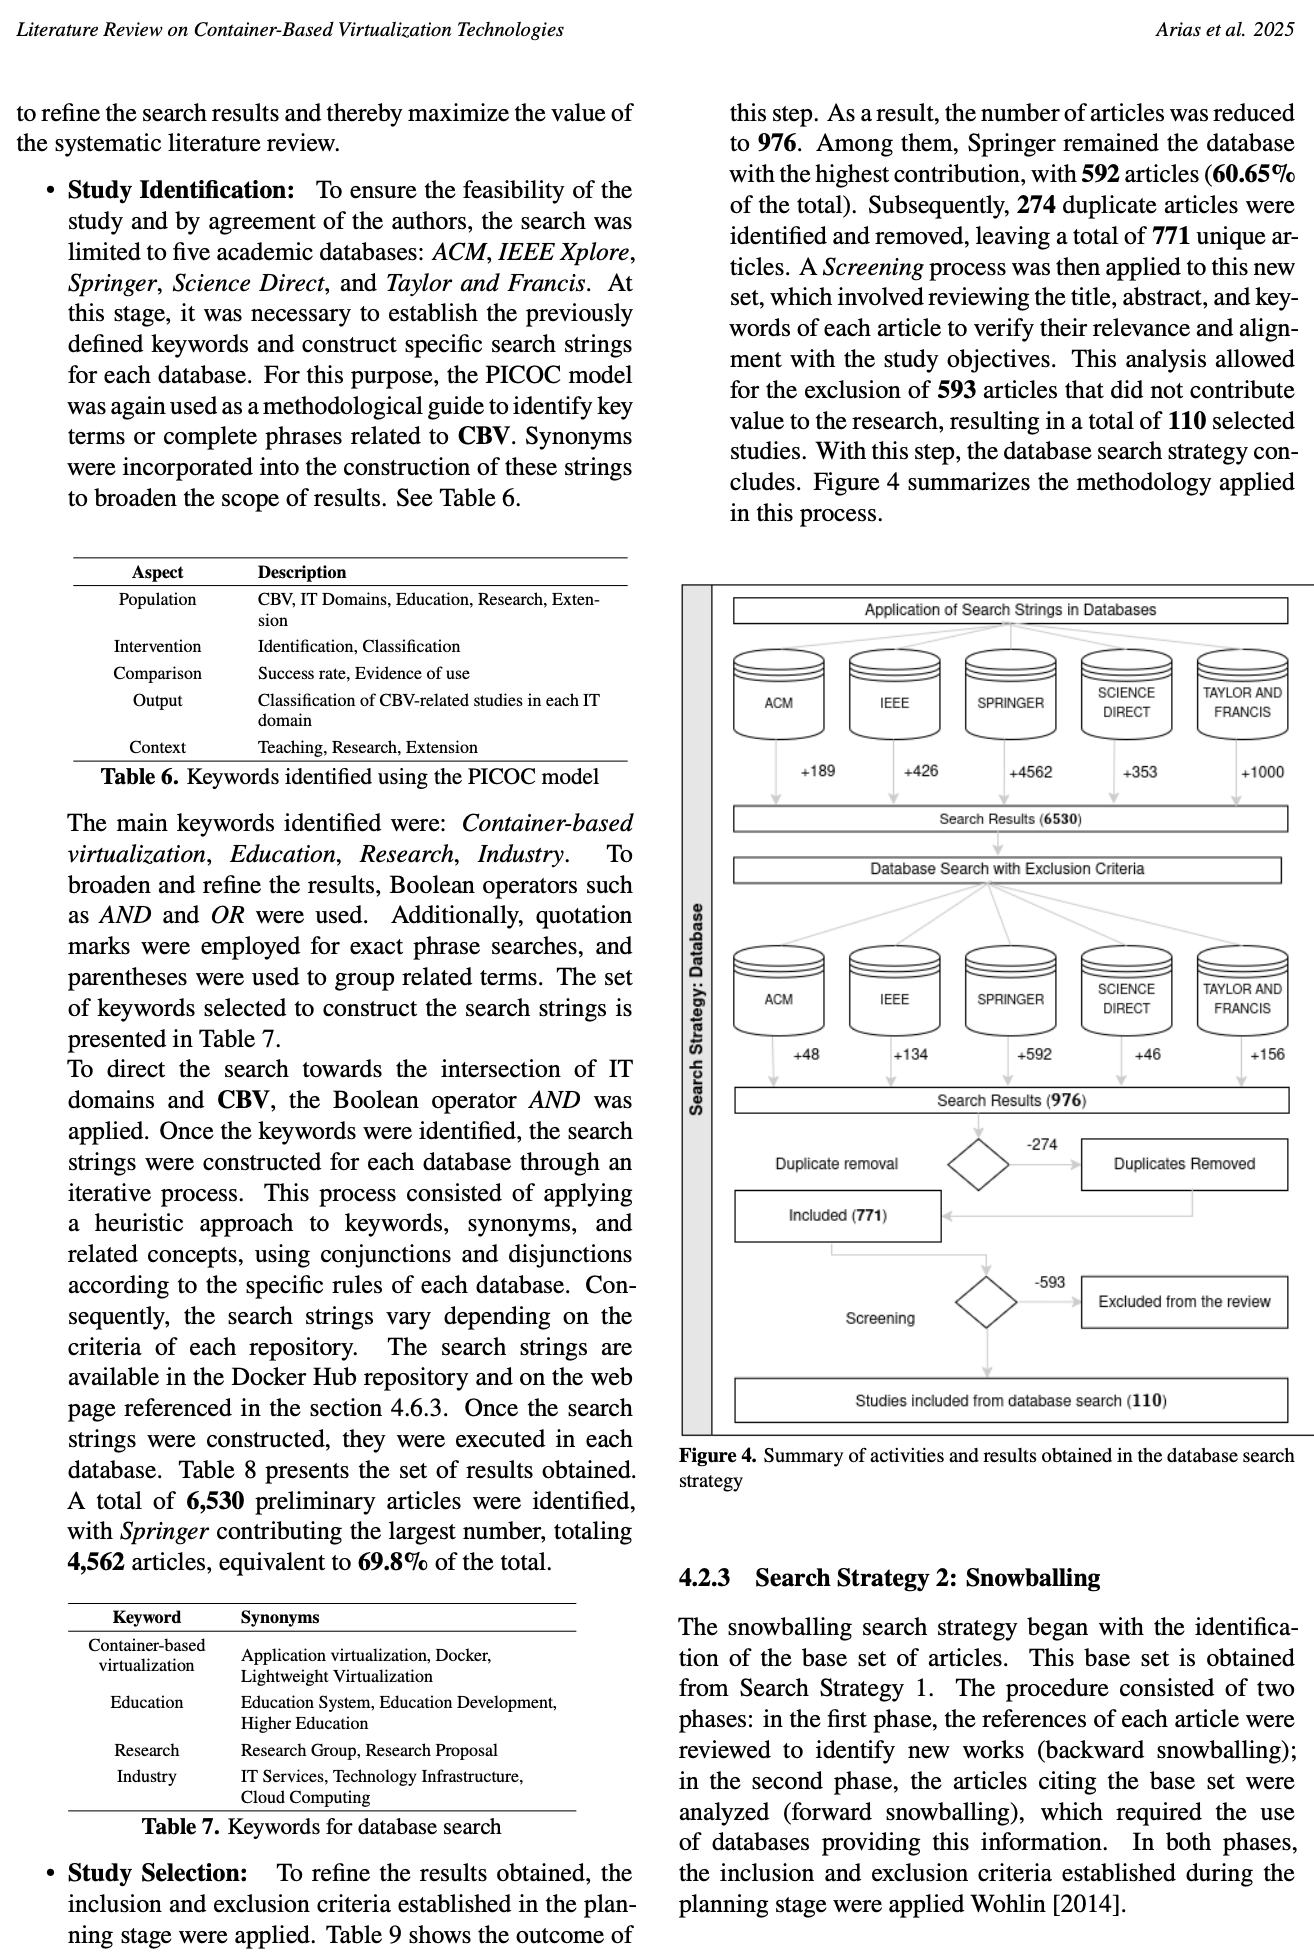
\includegraphics[width=0.95\textwidth,keepaspectratio]{apendices/JISA/pagina_5.png}
    \end{tcolorbox}
    \caption{Artículo JISA --- Página 5}\label{fig:jisa-pagina-5}
\end{figure}
\FloatBarrier% Macro para crear páginas del artículo de forma automática
% Páginas 6-34
\newcounter{jisampage}
\setcounter{jisampage}{6}
\loop%
    \begin{figure}[H]
        \centering
        \begin{tcolorbox}[
            colback=white,
            colframe=gray!50,
            boxrule=1pt,
            arc=2pt,
            boxsep=5pt,
            left=3pt,
            right=3pt,
            top=3pt,
            bottom=3pt,
            drop shadow
        ]
            \includegraphics[width=0.95\textwidth,keepaspectratio]{apendices/JISA/pagina_\thejisampage.png}
        \end{tcolorbox}
        \caption{Artículo JISA --- Página \thejisampage}\label{fig:jisa-pagina-\thejisampage}
    \end{figure}
    \FloatBarrier\stepcounter{jisampage}
    \ifnum\value{jisampage}<35
\repeat%

\section{Slides de CEIFI}
\foreach \n in {1,...,16} {
    \begin{figure}[H]
        \centering
        \fbox{\includegraphics[width=0.9\textwidth]{apendices/CEIFI/\n.png}}
        \caption{Slide \n de CEIFI}
    \end{figure}
}

\section{Slides de GRID 2025-I}
\foreach \n in {1,...,13} {
    \begin{figure}[H]
        \centering
        \fbox{\includegraphics[width=0.9\textwidth]{apendices/GRID-2025/\n.png}}
        \caption{Slide \n de GRID 2025-I}
    \end{figure}
}

\section{Poster GRID 2024-II}
\begin{figure}[H]
    \centering
    \fbox{\includegraphics[width=0.9\textwidth]{apendices/GRID-2024/image.png}}
    \caption{Póster de GRID 2024-II}
\end{figure}